\chapter{Portfolio Allocation}
\bichaptertitle{投资组合配置}

\audiencebox{Staunch systems trader / Asset allocating investor}{This chapter is about deciding how you share out your trading capital between different instruments or trading rules. Deciding the allocation between instruments is important for asset allocating investors, whilst staunch systems traders have to make both kinds of decision. It isn't relevant if you're a semi-automatic trader, since you won't use systematic trading rules and will trade different instruments opportunistically. You can skip this chapter.\par\medskip
坚定的系统化交易者 / 资产配置型投资者\par\medskip
本章讨论的是如何在不同品种或不同交易规则之间分配交易资本。
对资产配置型投资者而言，
最重要的是决定品种之间如何分配；
而坚定的系统化交易者则需要同时面对这两类配置决策。
如果你是半自动交易者，
由于你不会使用系统化交易规则，
而且会在不同品种之间机会性交易，
那么这一章与你关系不大，可以跳过。}

DECIDING HOW TO ALLOCATE WITHIN A PORTFOLIO OF ASSETS IS a problem every investor faces. How much in equities, bonds or cash? Should you split your equity allocation evenly between countries or just stick it all in the USA? Allocation decisions are equally important for systematic investors and traders. If you're a staunch systems trader running more than one trading rule, including any variations, then you need to decide what forecast weights to use when you combine rules together to forecast the price of each instrument. Both staunch systems traders and asset allocating investors also need to decide instrument weights; how much of your portfolio to put into the trading systems you have for each instrument. Because the tools in this chapter are for making both kinds of decision, I'll refer to portfolios of generic assets, which could be either instruments or trading rules. Later in the book I'll show you specific examples of each of the two types of allocation problem. Just like trading rules, portfolio weights can be over-fitted. Optimising weights can give you a portfolio which does really well in back-tests, but which fails badly when traded

in reality. Such portfolios are usually highly extreme; allocating to just a small subset of the assets available. In this chapter I'll show you how to avoid the pitfalls of these highly undiversified portfolios.

任何投资者都会面对一个问题：如何在一个资产组合内部进行配置。股票、债券和现金该各占多少？股票配置要不要平均分配到多个国家，
还是干脆全放在美国？对于系统化投资者和交易者来说，这类配置决策同样重要。如果你是一名运行着多条交易规则
（包括规则变体）的坚定系统化交易者，那么你就必须决定，在把这些规则组合起来预测每个品种价格时，
各条规则应当使用什么样的预测权重。坚定的系统化交易者和资产配置型投资者还都需要决定品种权重：你应该把整个投资组合的多少比例，
配置到每一个品种对应的交易系统中。由于本章中的工具同时适用于这两类决策，我会用“通用资产组合”来表述问题，而这些“资产”既可能是品种，也可能是交易规则。
本书后面我会分别给出这两类配置问题的具体示例。就像交易规则本身一样，投资组合权重也可能过拟合。优化权重可以给你一个在回测中表现极佳、
但在真实交易中彻底失效的投资组合。这样的投资组合通常都非常极端，只会把资金集中到极少数资产上。本章将展示如何避开这种高度不分散化组合的陷阱。

\section*{Chapter overview}
\phantomsection
\addcontentsline{toc}{section}{Chapter overview}
\bisectiontitle{本章概览}

\begin{tabularx}{\textwidth}{@{}p{0.30\textwidth}Y@{}}
\textbf{Optimising gone bad} & How classic portfolio optimisation can often result in over-fitted extreme portfolio weights. \\
\textbf{Saving optimisation from itself} & Some insights from an alternative technique, bootstrapping, which can help us understand what is going wrong. \\
\textbf{Making weights by hand} & How to use a simple method called handcrafting to get portfolio weights. \\
\textbf{Incorporating Sharpe ratios} & Using additional information about expected performance to improve handcrafted weights. \\
\end{tabularx}

\medskip

\begin{tabularx}{\textwidth}{@{}p{0.30\textwidth}Y@{}}
\textbf{优化为何会变坏} & 经典投资组合优化为何经常会导出过拟合的极端权重。 \\
\textbf{如何拯救优化本身} & 使用另一种技术 bootstrapping 所带来的洞见， 帮助我们理解优化到底出了什么问题。 \\
\textbf{如何手工做权重} & 怎样使用一种叫 handcrafting 的简单方法来得到组合权重。 \\
\textbf{纳入夏普比率} & 如何利用关于预期表现的额外信息来改进手工权重。 \\
\end{tabularx}

\section*{Optimising gone bad}
\phantomsection
\addcontentsline{toc}{section}{Optimising gone bad}
\bisectiontitle{优化为何会变坏}

\subsection*{Introducing optimisation}
\bisubsectiontitle{优化是什么}

Portfolio optimisation will find the set of asset weights which give the best expected risk adjusted returns, usually measured by Sharpe ratio. The inputs to this are the expected average returns, standard deviation of returns, and their correlation. The standard method for doing this was first introduced by Harry Markowitz in the 1950s. It was a neat and elegant solution to a complex problem. Unfortunately it's all too easy to be distracted by elegance, and forget the important assumptions underlying the maths. As you will see below, blind use of this method frequently results in ugly portfolios with extreme weights. Just because an equation is wonderful to behold doesn't mean you should slavishly use its results without thought of the consequences. As Einstein said, "If you are out to describe the truth, leave elegance to the tailor." In the early part of my career I was fatally distracted by the lovely equations and ended up with some terrible portfolios, until I learned the error of my ways. Subsequently I often had to review the allocation decisions made by researchers who were less experienced, although undoubtedly cleverer and more academically qualified than myself.

When I asked one of these rocket scientists what they thought about the extreme portfolio weights they'd found I often got a shrug. "These are what the optimiser came up with." The unspoken assumption was that the equation must be right. Hopefully after reading this chapter you will be less accepting of attractive mathematics.

投资组合优化试图找出那组资产权重，使得组合的预期风险调整后收益最大，通常这个目标会用夏普比率来度量。它所依赖的输入，是资产的预期平均收益、
收益标准差以及它们之间的相关性。完成这件事的标准方法，最早由 Harry Markowitz 在 20 世纪 50 年代提出。它是一个优雅而简洁的数学解法。
遗憾的是，人们太容易被这种优雅吸引，而忘记了支撑这套数学背后的关键假设。你很快会看到：如果盲目使用这种方法，
它往往会给出一些极其丑陋的投资组合
--- 权重非常极端、集中度极高。一个公式看起来再漂亮，也不意味着你就应该在完全不考虑后果的情况下，对它俯首帖耳。
正如爱因斯坦所说：“如果你追求真理，就把优雅留给裁缝吧。”在我职业生涯早期，我也曾被这些漂亮方程严重误导，结果构造出一些糟糕透顶的组合，
直到后来我才认识到自己的错误。再后来，我又经常需要去审阅一些研究员所做的配置决策
--- 他们也许比我更聪明、学历更高，但经验却更少。

\subsection*{Some good news}
\bisubsectiontitle{一点好消息}

Portfolio optimisation is hard. But there are a few difficulties that don't arise when you're using it to design trading strategies. This is because you aren't deciding directly how large your positions in various instruments should be. Instead you're deciding what weight should be given to different parts of your trading system. These can either be the forecast weights telling you in what proportion to use trading rule variations for a particular instrument, or the instrument weights determining how much of your capital to allocate for trading each instrument. This gives you two advantages. Firstly, you can't have negative weights in your portfolio; you can't short trading rules, so the lowest possible weight is zero. If a trading rule is expected to lose money you shouldn't include it at all.56 Secondly, using my framework will mean that profits from your trading rules have identical expected standard deviation of returns. This is because of the volatility standardisation I spoke about in chapter two, ‘Systematic Trading Rules'. By using this technique you simplify the problem and only need to use expected Sharpe ratios and correlations to work out your weights. Although you won't be optimising the underlying positions in individual assets like equities or bonds in your trading systems, I will be using portfolios of simple assets in this chapter to make the examples more straightforward. However to make it easier to interpret the results I will adjust asset returns before any calculations so that they have the same standard deviation as you'll have when you work with trading system returns.

投资组合优化很难，但在用它设计交易系统时，有几个困难其实会自然消失。原因是：你并不是在直接决定某个品种最终应当持有多大仓位，
而是在决定交易系统不同部分各自应该分到多少权重。这些权重既可能是预测权重
（决定某个品种上不同交易规则变体该如何混合），也可能是品种权重
（决定你的资本该分配到每个品种对应的子系统上多少）。这带来了两个好处。第一，你不需要允许负权重；
交易规则本身不能被“做空”，因此它们的最低权重天然就是零。如果一条交易规则预期会亏钱，你压根就不应该把它纳入组合。56
第二，在我的框架中，交易规则产生的收益已经完成了波动率标准化，因此它们具有相同的预期收益标准差。于是，问题被大大简化了：
你只需要关心预期夏普比率和相关性，而不必同时处理一堆不同波动率的资产。虽然在这一章里，你最终并不是直接去优化股票或债券本身的持仓规模，
但为了让例子更直观，我仍然会用简单资产组合来说明原理。为了便于解释结果，我也会在计算前先把这些资产的收益都调整到相同标准差。

\subsection*{The unstable world of portfolio weights}
\bisubsectiontitle{不稳定的组合权重世界}

Let's take a simple example of allocating capital between three assets: the NASDAQ and S\&P 500 US stock indices, and the US 20 year benchmark bond. I am using data from January 1999 to mid-2014 and all returns are volatility standardised to have the same expected standard deviation. Each year from January 2000 onwards I'm going to use returns from all previous years to calculate some optimal weights.\footnote{If you read the previous chapter you should recognise this as an out of sample expanding window.\par 如果你读过前一章，
你应该能认出这就是一种样本外 expanding window。} Because each optimisation uses all available data to create a single set of weights I call this a single period optimisation.

\begin{enumerate}
  \item A rule with a significantly negative Sharpe ratio either has very high trading costs and should be omitted, or it is consistently wrong and so should be inverted with longs and shorts reversed before incorporating it into the portfolio (although you'll probably also want to consider the logic of your original idea before proceeding).
\end{enumerate}

The calculation is done using the classic Markowitz optimisation; I find the maximum risk adjusted return (e.g. Sharpe ratio) using the estimated means and correlations, and standard deviations (which are all identical because I've used volatility standardisation). I also don't allow weights to be negative and they have to sum up to exactly 100\%. Figure 14 shows the weights calculated for each year.\footnote{Remember these are displayed as if all assets had the same standard deviation. So in practice roughly twice as much actual money would be allocated to bonds than shown here, due to their lower volatility.\par 记住，这里的展示是假设所有资产都拥有相同标准差。
因此在真实资金分配中，由于债券波动率更低，它所对应的实际现金配置通常会比图中所示高出约一倍。} In the last throes of the late 1990s tech boom I naturally put all my money into the fast rising NASDAQ. This then implodes, and is permanently removed from the portfolio. For much of the remaining period I put my entire capital in bonds. At the end I only have 25\% in equities, all of which is in the S\&P 500. This is a very extreme portfolio, with very unstable weights.

\begin{figure}[htbp]
  \centering
  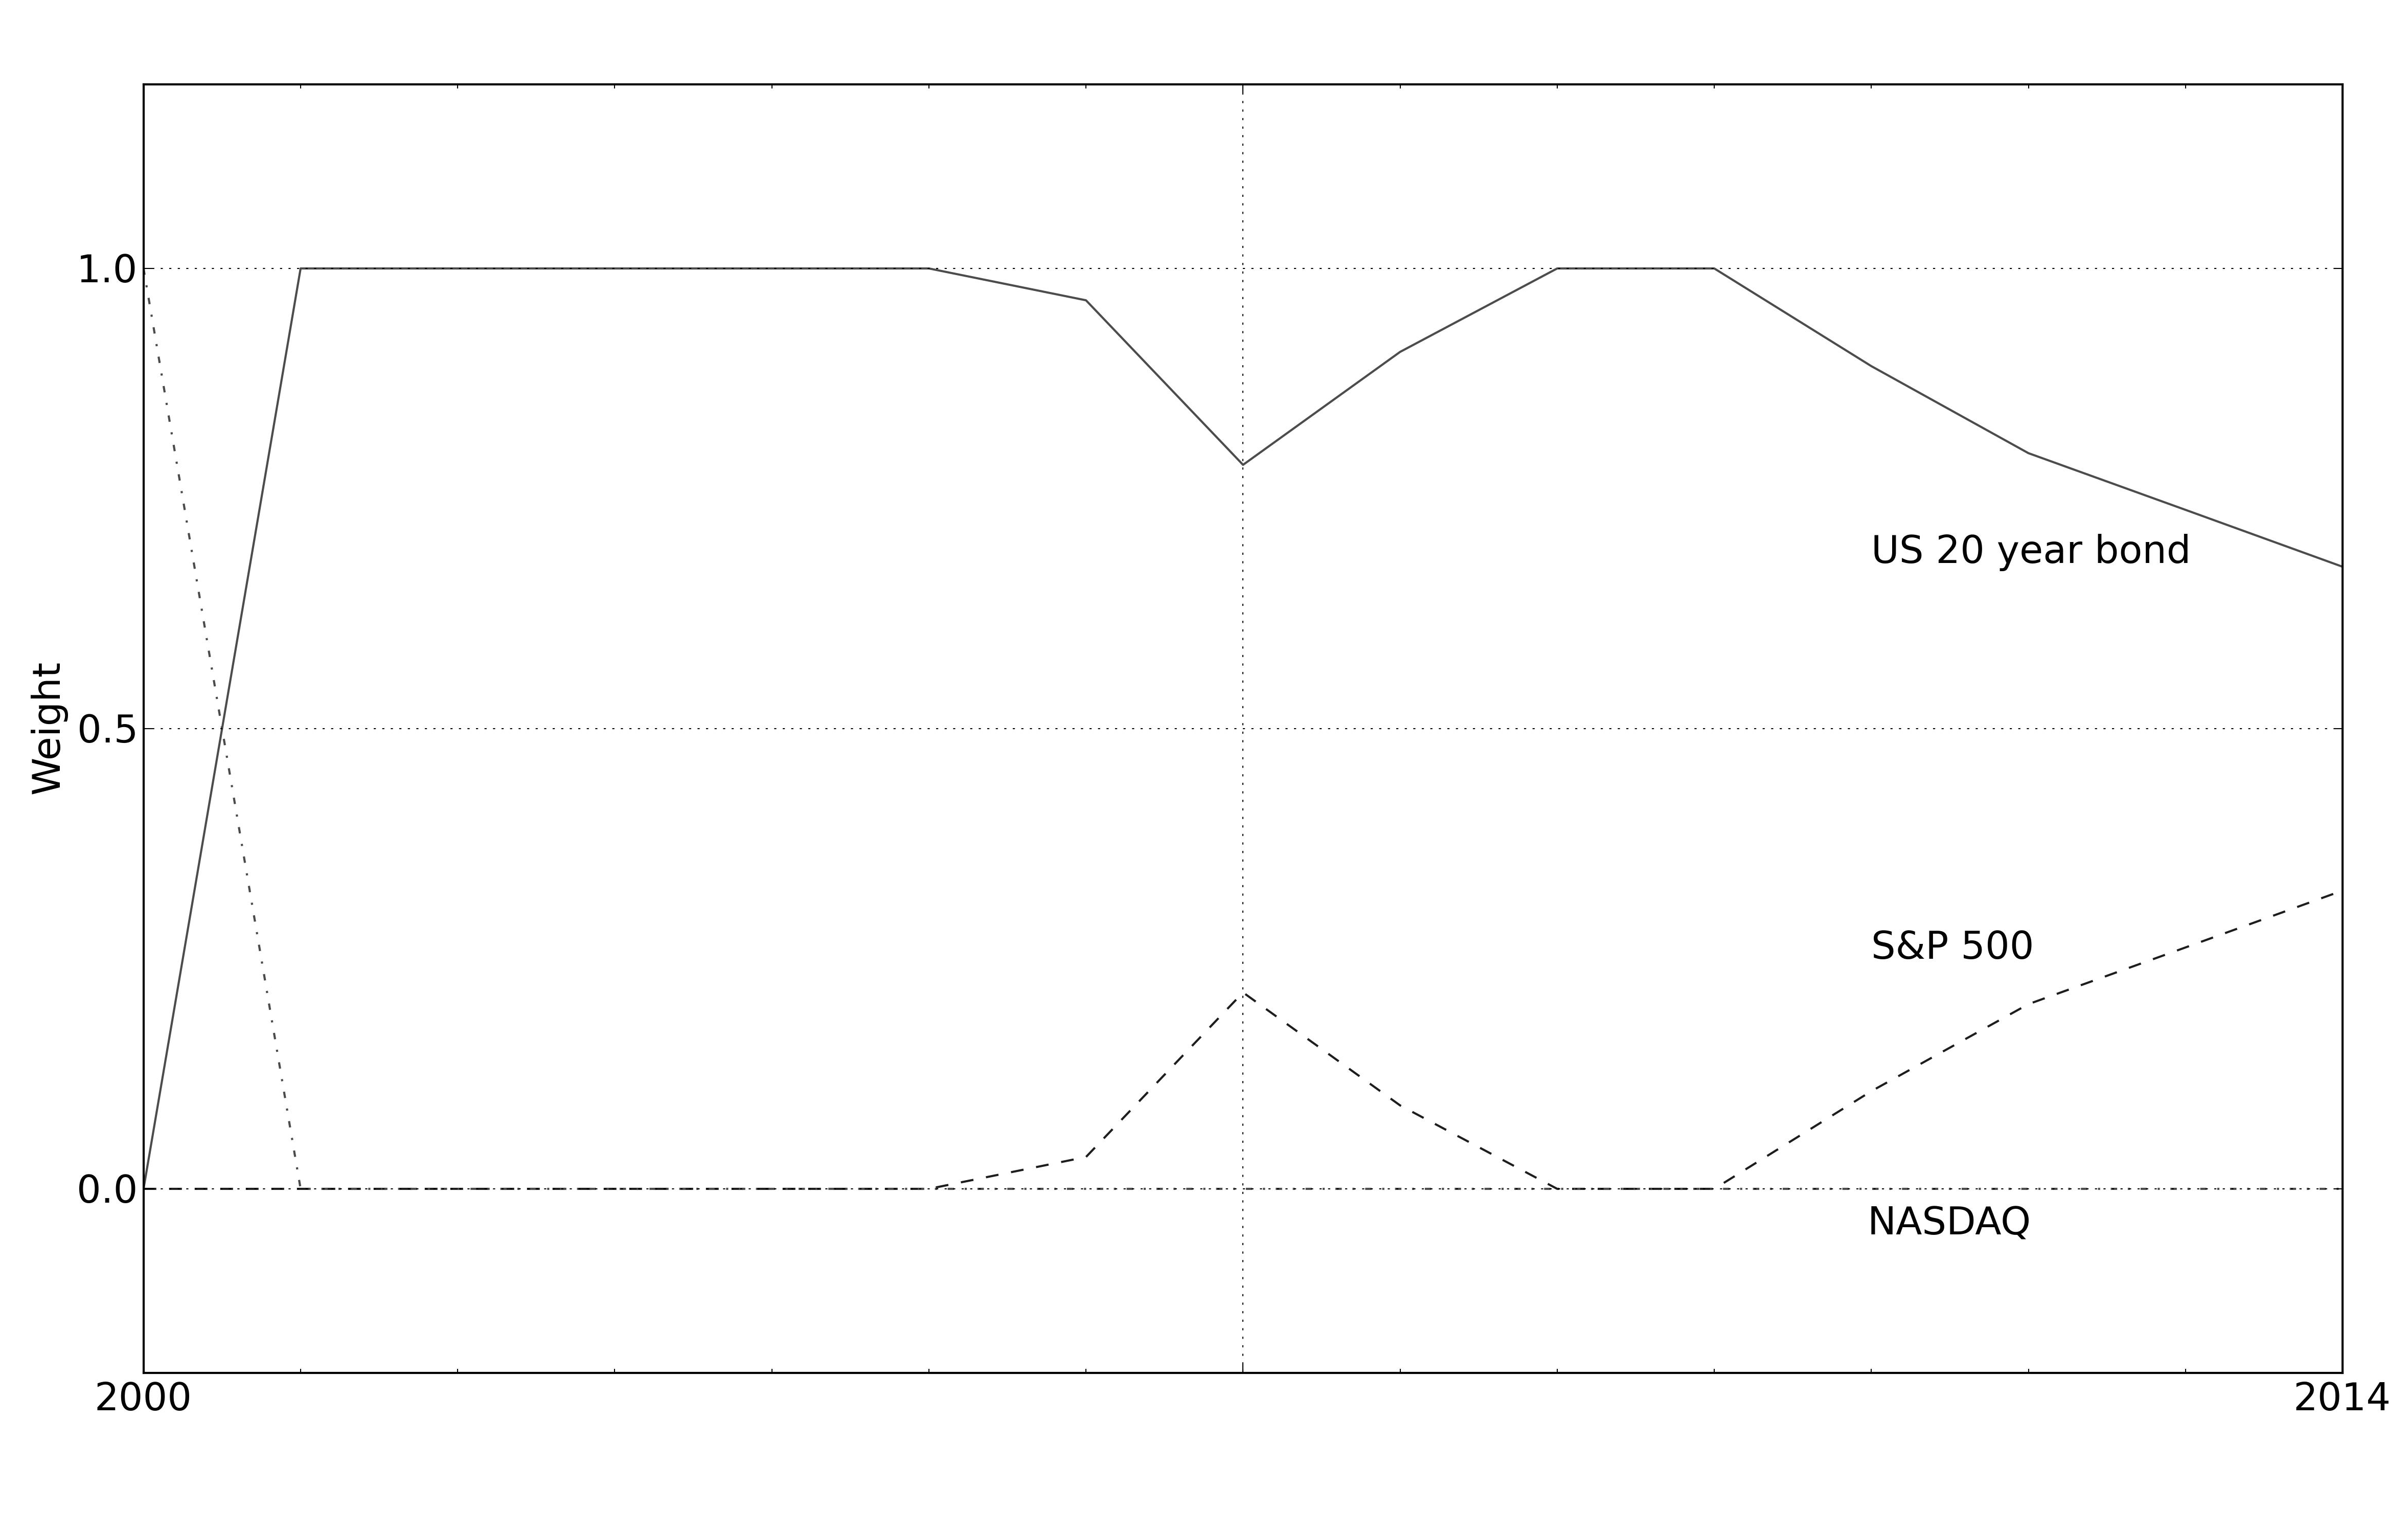
\includegraphics[width=\textwidth]{figures/raw/img-014.png}
  \caption{SINGLE PERIOD OPTIMISATION USUALLY MEANS EXTREME WEIGHTS\\
  单期优化通常意味着极端权重}
\end{figure}

The figure shows the portfolio weights produced by single period optimisation done each year on all previous data.

我们来看一个简单例子：在 NASDAQ、S\&P 500 和美国 20 年期国债之间分配资本。我使用 1999 年 1 月到 2014 年中期的数据，
并把所有收益都做了波动率标准化，使它们拥有相同的预期标准差。然后，从 2000 年开始的每一年，我都用此前全部历史数据去算一次最优权重。
由于每次优化都基于“到当时为止的全部样本”来给出一套权重，这种做法被称为单期优化
（single period optimisation）。

结果非常糟糕：在 1990 年代末科技泡沫最后疯狂阶段，组合几乎全仓 NASDAQ；随后 NASDAQ 崩溃，又被永久地剔除出去；
之后组合又长期几乎全仓债券；最后，股票只剩 25\%，而且全部集中在 S\&P 500 上。
这正是那种你一眼就能看出“完全不对劲”的极端组合：权重不稳定，而且过度集中。

\subsection*{Not all statistical estimates are created equal}
\bisubsectiontitle{不是所有统计估计都同样可靠}

Faced with such nightmares a natural reaction is to discard any hope of optimising. Perhaps we should just allocate equally to all the assets we have. Many academic researchers have

面对这样的噩梦，一个很自然的反应是彻底放弃优化：也许，我们干脆把所有资产都等权配置就好了。很多学术研究者也确实得出了类似结论。

also come to this conclusion and there is plenty of evidence that equal weights are hard to beat.59

\subsection*{When do equal weights make sense?60}
\bisubsectiontitle{什么时候等权配置是合理的？60}

\begin{enumerate}
  \item Same volatility: If all assets had the same expected standard deviation of returns. This is always the case for the volatility standardised assets we're using.
  \item Same Sharpe ratio: If all assets had the same expected Sharpe ratio (SR).
  \item Same correlation: If all assets had the same expected co-movement of returns. If these assumptions aren't correct, then what should your portfolio look like?61
\end{enumerate}

\begin{enumerate}
  \item 相同波动率：如果所有资产拥有相同的预期收益标准差。对我们这里已经完成波动率标准化的资产来说，这一点天然成立。
  \item 相同夏普比率：如果所有资产拥有相同的预期夏普比率
  （SR）。
  \item 相同相关性：如果所有资产之间的预期协同波动程度也相同。
\end{enumerate}

What kind of portfolio should we have with...

\begin{enumerate}
  \item Same Sharpe ratio and correlation: Equal weights.
  \item Significantly different Sharpe ratio (SR): Larger weights for assets that are expected to have higher SR, smaller for low SR.
  \item Significantly different correlation: Larger weights for highly diversifying assets which have lower correlations to other assets, and smaller for less diversifying assets. Let's see if these assumptions are true in the simple example. Figure 15 shows the distribution of Sharpe ratios for each of the three assets. Notice that the lines mostly overlap; this means we can't distinguish between the historic performance of each asset. Although bonds did have a higher average SR the advantage isn't statistically significant. If you read the previous chapter, and remember table 6, it is no surprise that the 15 years of data isn't enough to say with confidence which asset had the best SR.
  \item For example see DeMiguel, Victor, Lorenzo Garlappi and Raman Uppal, ‘Optimal versus naive diversification: How inefficient is the 1/N portfolio strategy?', Review of Financial Studies 2009.
  \item To be pedantic there are some unusual portfolios where equal weights are optimal that don't fulfill these criteria, but they aren't relevant here.
\end{enumerate}

\begin{figure}[htbp]
  \centering
  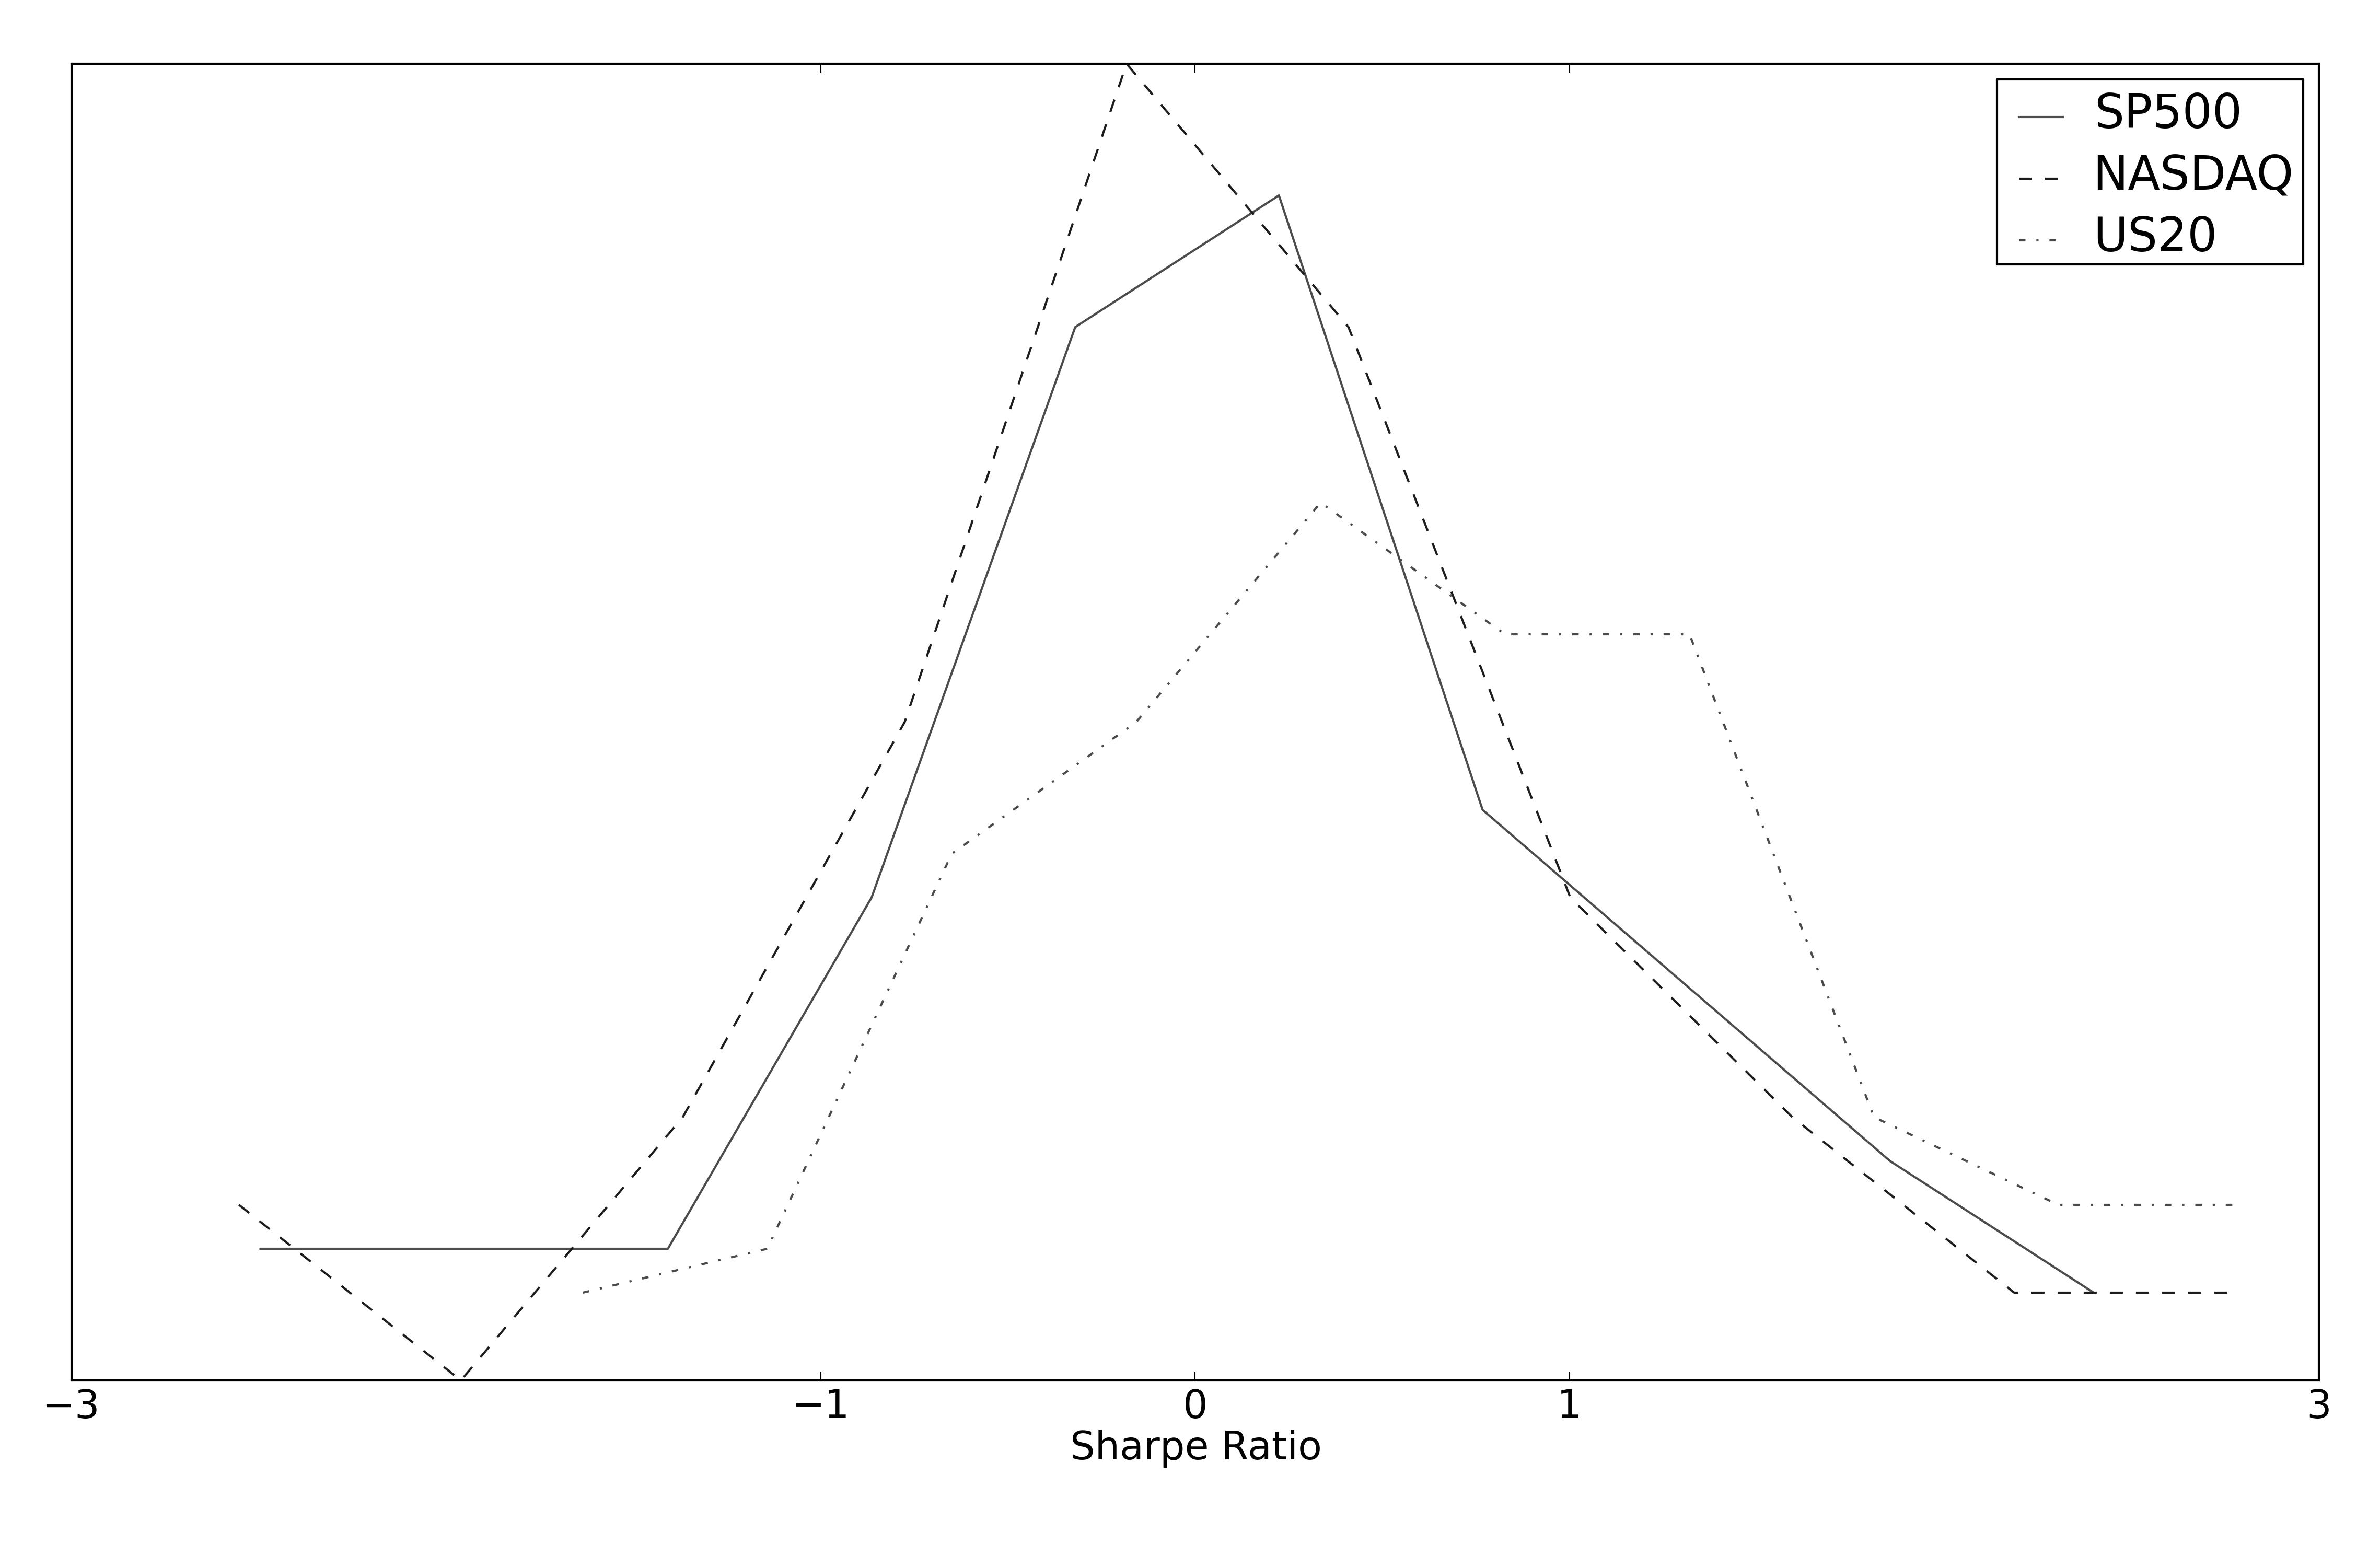
\includegraphics[width=\textwidth]{figures/raw/img-015.png}
  \caption{HARDER TO DISTINGUISH SHARPE RATIOS THAN YOU THINK\\
  区分不同夏普比率，比你想象中更难}
\end{figure}

\begin{figure}[htbp]
  \centering
  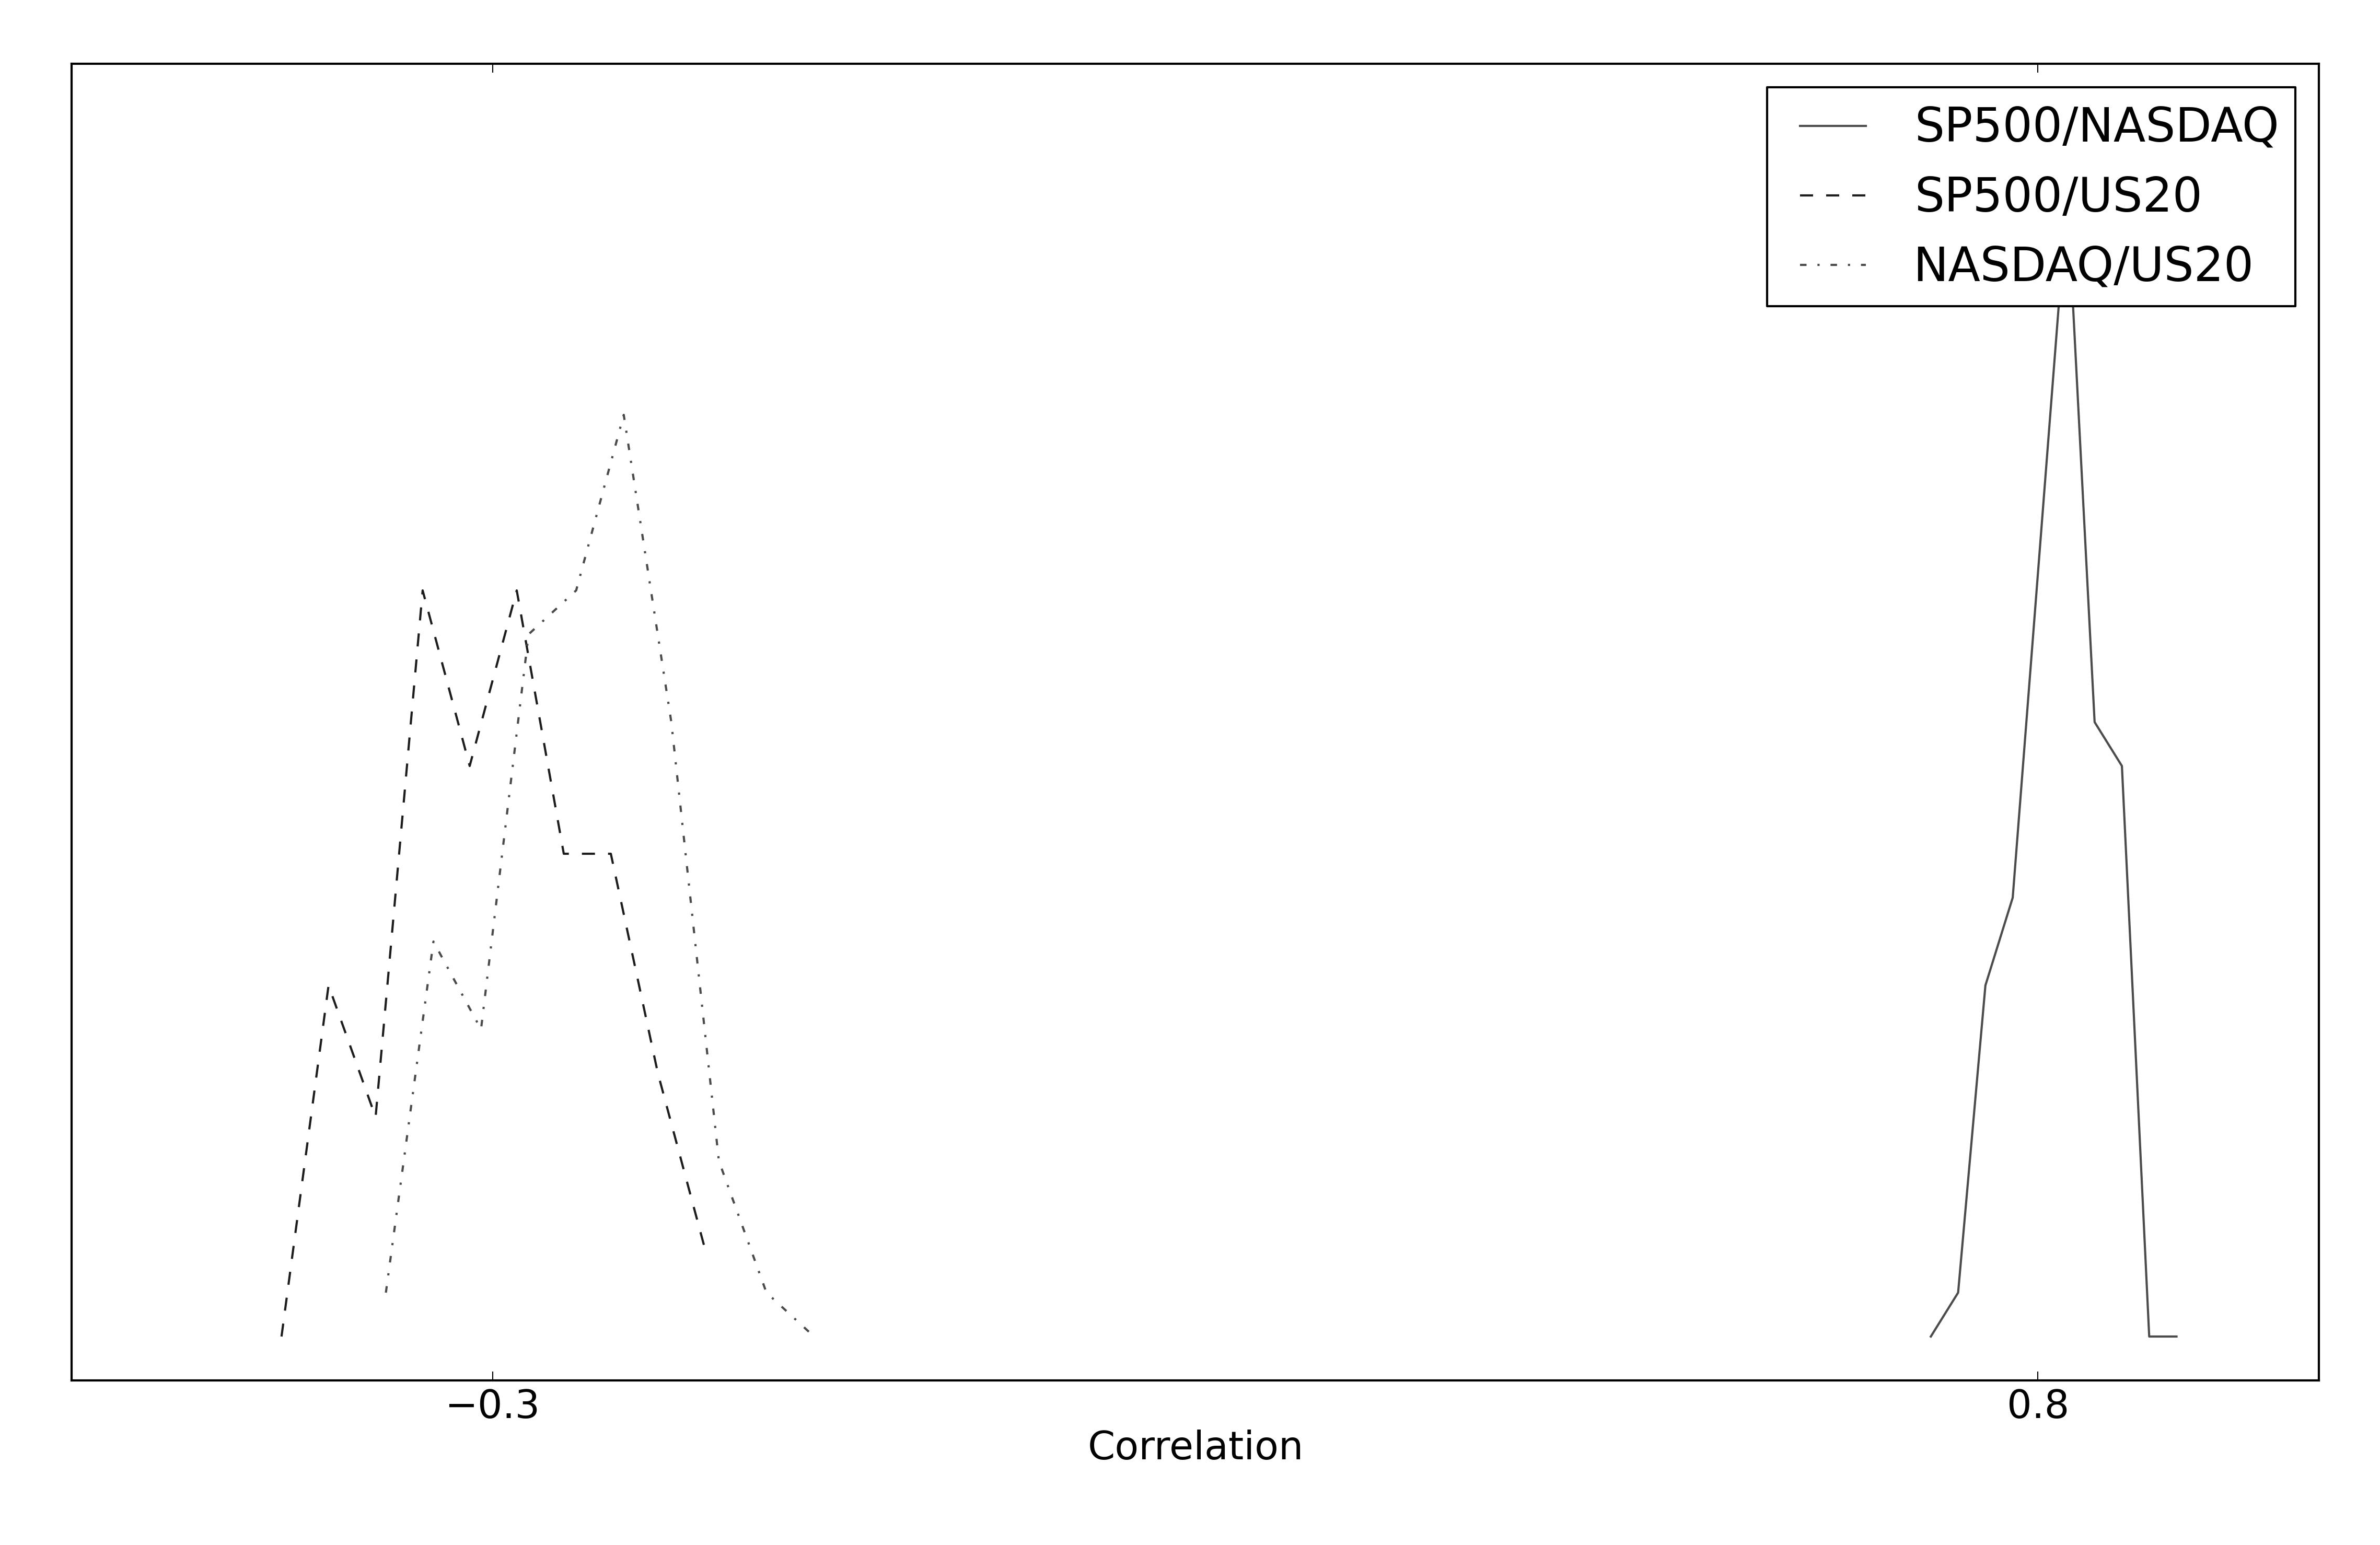
\includegraphics[width=\textwidth]{figures/raw/img-016.png}
  \caption{EQUITIES CLEARLY CORRELATED WITH EACH OTHER, AND NEGATIVELY WITH BONDS\\
  股票彼此之间明显相关，而与债券则呈负相关}
\end{figure}

The figure shows the distribution of correlations for pairs of the three assets in my example portfolio.

关键问题不在于“等权是不是看起来很蠢”，而在于：哪些统计量你真的能有把握地区分出来，哪些你其实分不出来。
在这个简单例子里，
夏普比率看上去有差异，
但并没有统计显著性；
而相关性差异却很清楚：
两只股票彼此高度相关，
而债券明显更具分散化价值。

因此，一个合理组合应当主要依据“可被可信识别的相关性差异”来偏离等权，
而不是根据那些样本不足以支撑的 Sharpe 差异来大幅押注。
可惜，经典优化器并不懂“估计的置信度”这件事。
它只看均值，
不看这些均值有多不可靠。

\section*{Saving optimisation from itself}
\phantomsection
\addcontentsline{toc}{section}{Saving optimisation from itself}
\bisectiontitle{如何拯救优化本身}

How can we fix this problem? I have two techniques that I use. The first, which is quite hard work, is called bootstrapping. This involves repeating my optimisation many times over different parts of the data, taking the resulting weights, and averaging them out. So the weights are the average of many optimisations, rather than one optimisation on the average of all data. The justification for bootstrapping is simple. I believe that the past is a good guide to the future, but I don't know which part of the past will be repeated. To hedge my bets I assume there is an equal chance of seeing any particular historical period repeated. So it's logical to use an average of all the portfolios which did best in previous periods. Bootstrapping has some nice advantages over classic optimisation. Most of the individual optimisations have extreme weights. However with enough of them it's unlikely the average will be extreme. If I have noisy data, and the past contains periods which were very different, then the optimal portfolios will be close to equal weights. But with significant differences in Sharpe ratios or correlations similar portfolios will crop up repeatedly,

那该如何修复这个问题？我自己主要使用两种技术。第一种相对更费工夫，叫 bootstrapping。它的做法是：
在数据的不同片段上反复执行优化，把每次得到的权重收集起来，再做平均。
也就是说，最终权重不再是“对所有数据均值做一次优化”的结果，
而是“对许多不同历史片段分别优化，再把这些优化结果平均”的结果。
它背后的逻辑其实很简单：
我相信过去可以为未来提供线索，
但我并不知道未来究竟会更像过去的哪一段。
既然如此，
我就假设过去的任何一个时期都可能重新出现，
那么最自然的做法，就是把这些历史时期中“表现最好”的组合都考虑进来，再取它们的平均。
相比经典优化，bootstrapping 有一个非常漂亮的优点：
单次优化往往都会给出极端权重，
但只要你做足够多次，
它们的平均结果通常就不会极端。

and the average will reflect that. The averaged weights naturally reflect the amount of uncertainty that the data has. Let's see the results of running an expanding window bootstrap optimisation on our simple three asset portfolio. Figure 17 shows the results over time, whilst table 7 compares the final weights with a classic single period optimisation and equal weights.\footnote{This is the result of using 100 bootstraps, each 1 year in length, with daily returns drawn randomly with replacement.\par 这里的结果来自 100 次 bootstrap，
每次抽取长度为 1 年的样本，
并对日收益做有放回随机抽样。} After the first year the weights are relatively stable, and for all periods less extreme than for the single period method. However the diversifying allocation to bonds is greater than with equal weights, so this portfolio should do better.

\begin{figure}[htbp]
  \centering
  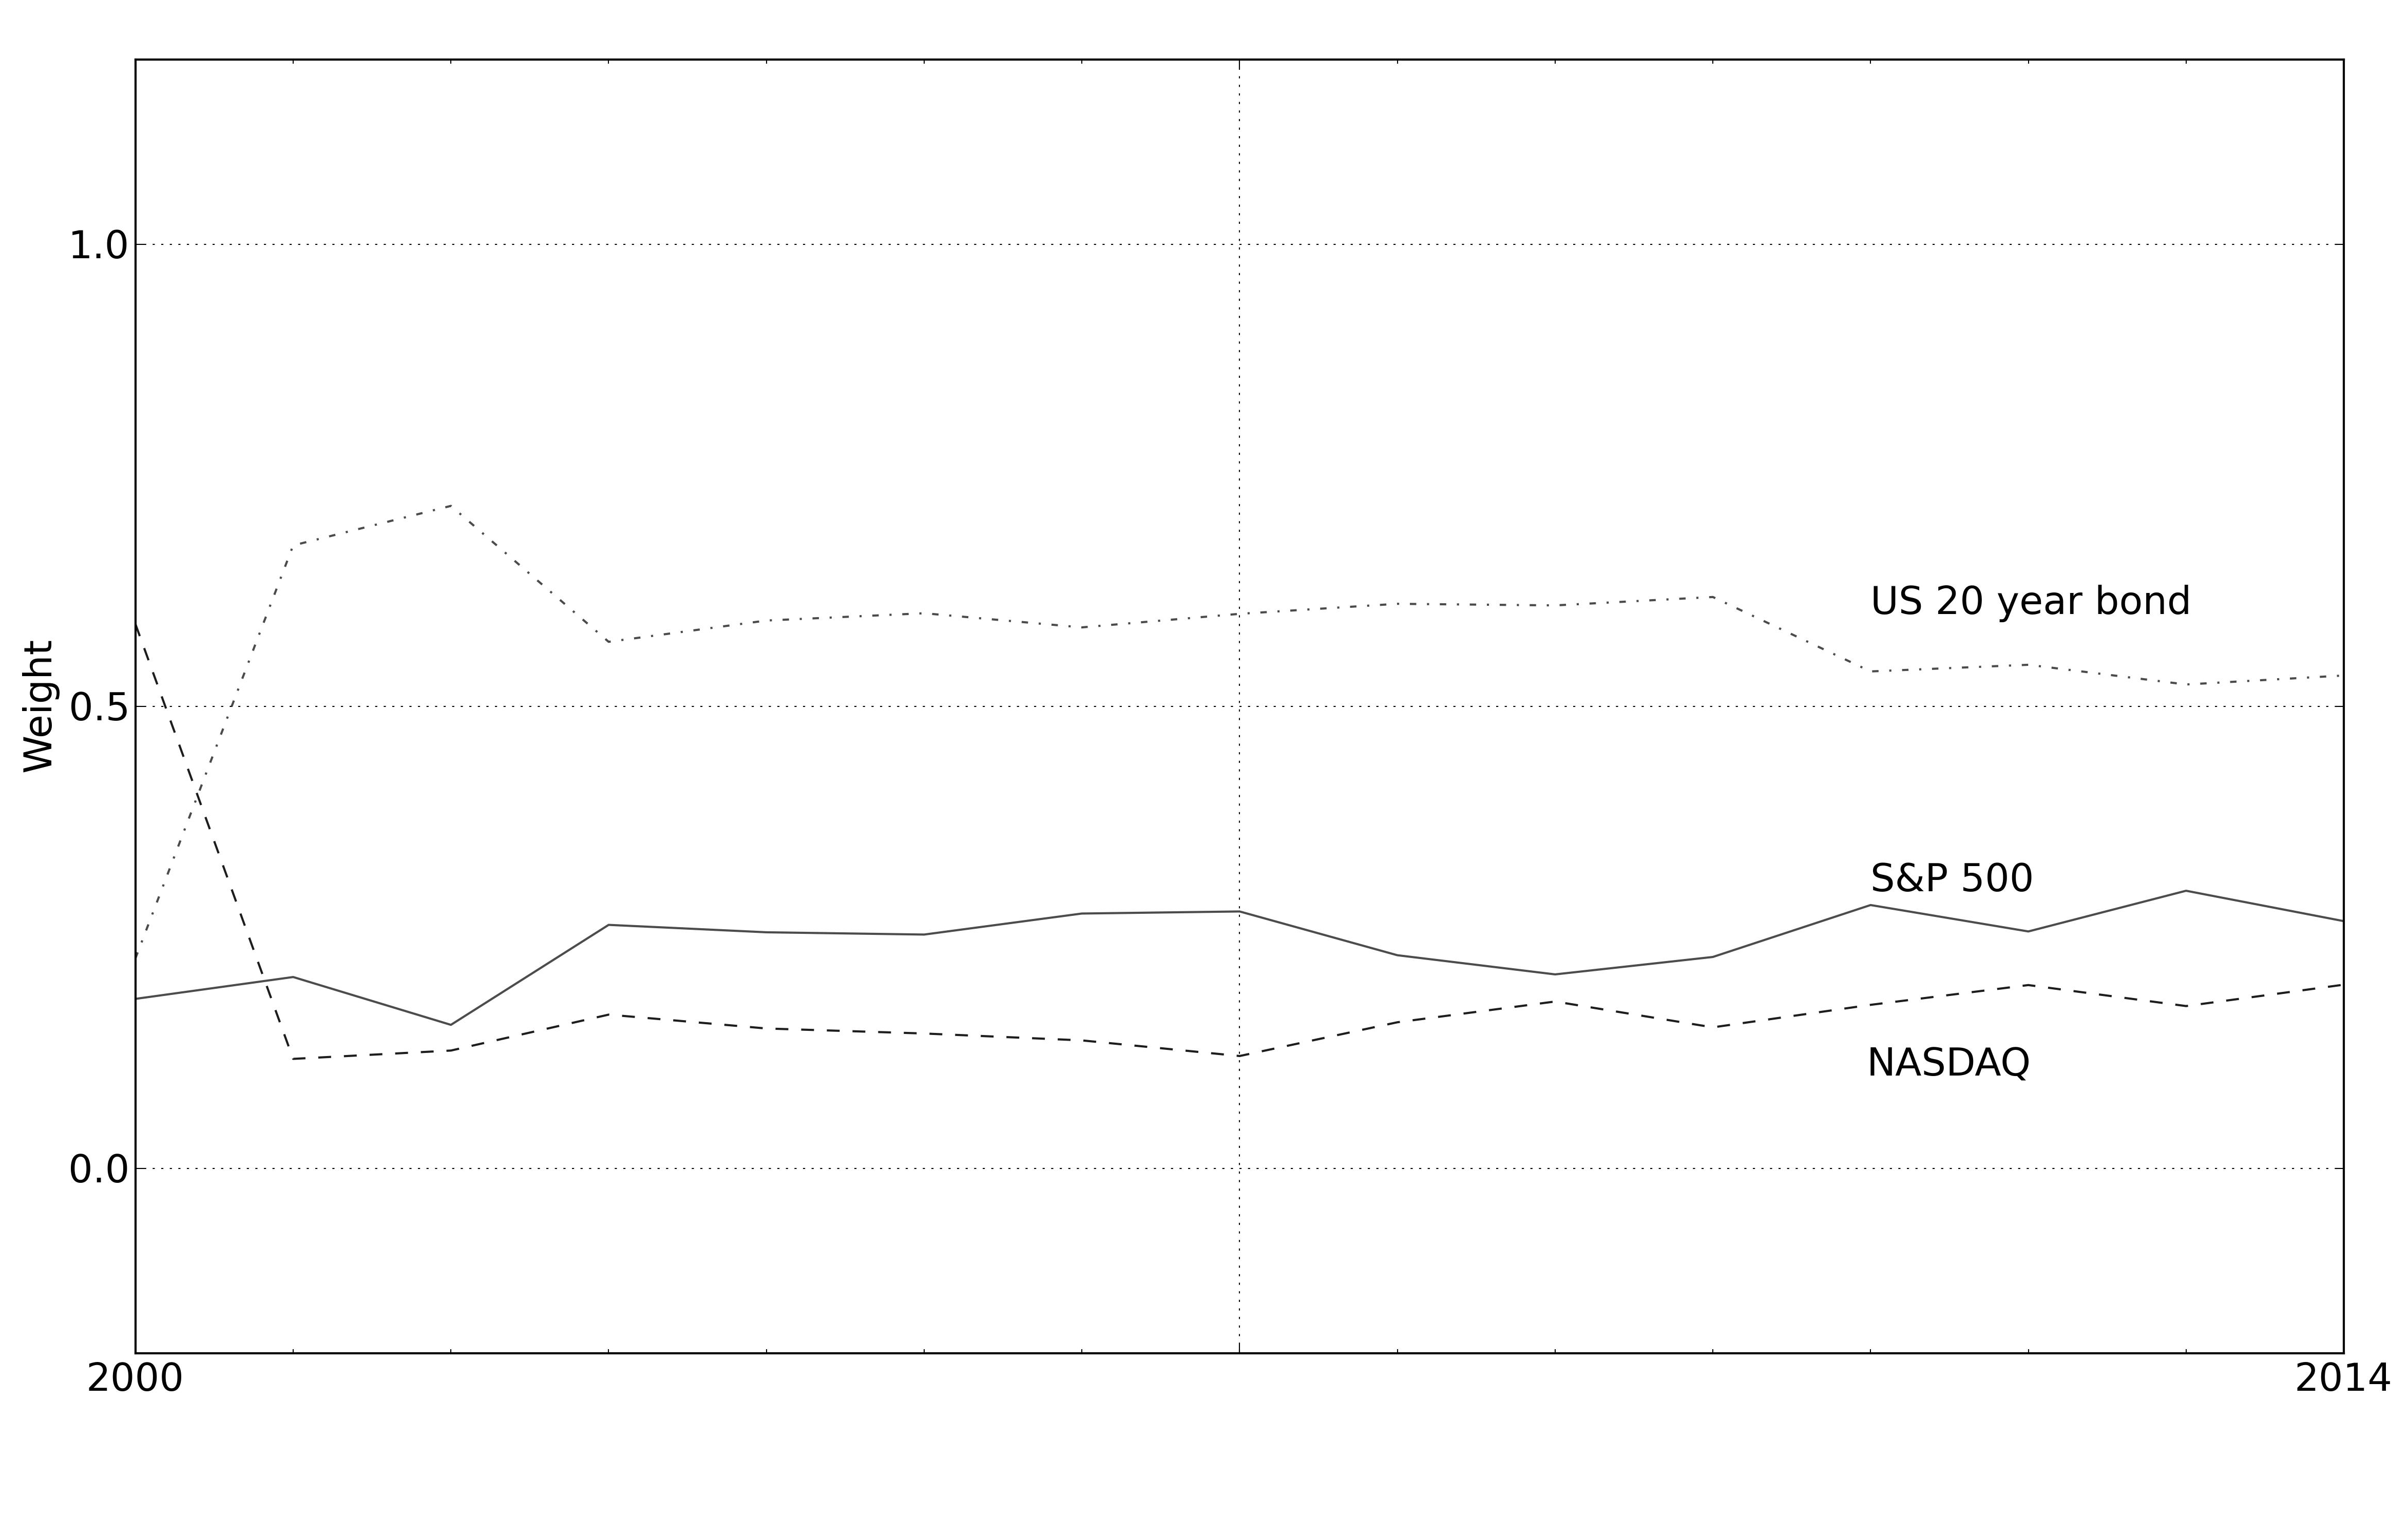
\includegraphics[width=\textwidth]{figures/raw/img-017.png}
  \caption{BOOTSTRAPPED PORTFOLIO WEIGHTS: STABLE AND EVENLY SPREAD\\
  Bootstrapped 组合权重：稳定且分布均匀}
\end{figure}

The figure shows the distribution of correlations for pairs of the three assets in my example portfolio.

\section*{Saving optimisation from itself}
\phantomsection
\addcontentsline{toc}{section}{Saving optimisation from itself}

How can we fix this problem? I have two techniques that I use. The first, which is quite hard work, is called bootstrapping. This involves repeating my optimisation many times over different parts of the data, taking the resulting weights, and averaging them out. So the weights are the average of many optimisations, rather than one optimisation on the average of all data. The justification for bootstrapping is simple. I believe that the past is a good guide to the future, but I don't know which part of the past will be repeated. To hedge my bets I assume there is an equal chance of seeing any particular historical period repeated. So it's logical to use an average of all the portfolios which did best in previous periods. Bootstrapping has some nice advantages over classic optimisation. Most of the individual optimisations have extreme weights. However with enough of them it's unlikely the average will be extreme. If I have noisy data, and the past contains periods which were very different, then the optimal portfolios will be close to equal weights. But with significant differences in Sharpe ratios or correlations similar portfolios will crop up repeatedly,

and the average will reflect that. The averaged weights naturally reflect the amount of uncertainty that the data has. Let's see the results of running an expanding window bootstrap optimisation on our simple three asset portfolio. Figure 17 shows the results over time, whilst table 7 compares the final weights with a classic single period optimisation and equal weights.\footnote{This is the result of using 100 bootstraps, each 1 year in length, with daily returns drawn randomly with replacement.} After the first year the weights are relatively stable, and for all periods less extreme than for the single period method. However the diversifying allocation to bonds is greater than with equal weights, so this portfolio should do better.

\begin{figure}[htbp]
  \centering
  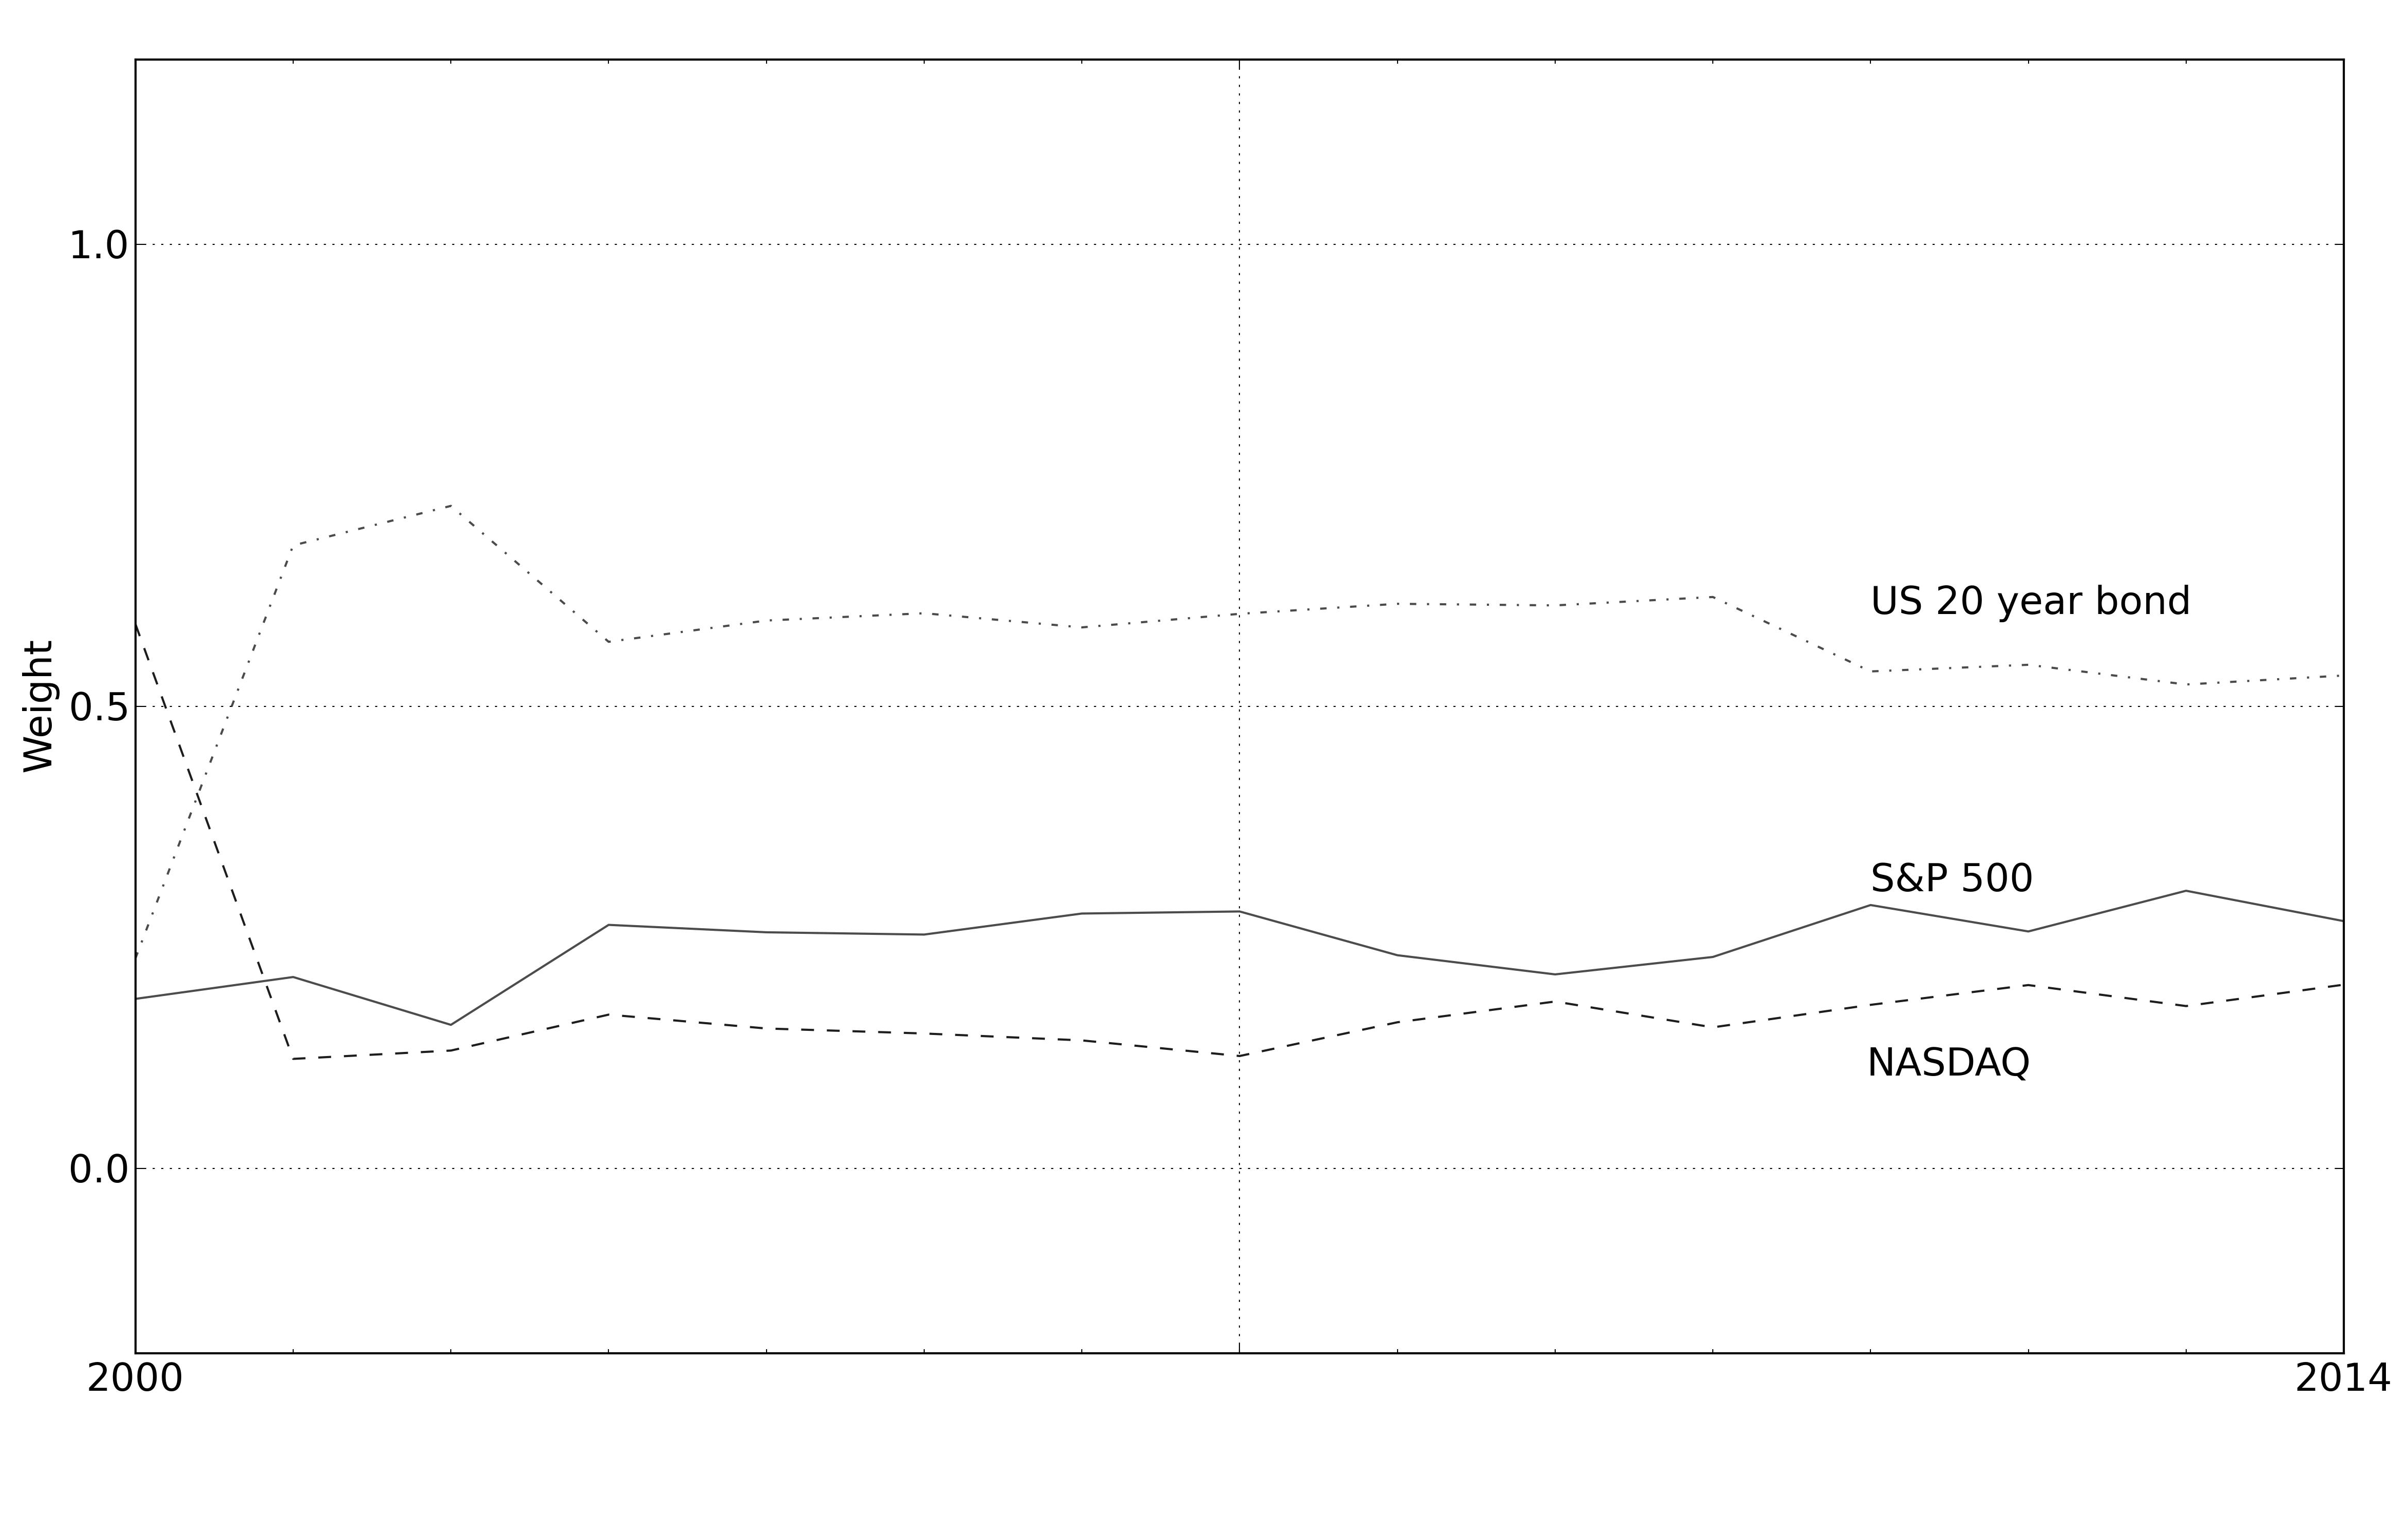
\includegraphics[width=\textwidth]{figures/raw/img-017.png}
  \caption{BOOTSTRAPPED PORTFOLIO WEIGHTS: STABLE AND EVENLY SPREAD}
\end{figure}

The figure shows the portfolio weights I get over time from using the bootstrap method on the example assets.

\rawtablecaption{BOOTSTRAPPED WEIGHTS ARE MORE EVEN THAN THE SINGLE PERIOD METHOD, BUT ACCOUNT FOR CORRELATIONS BETTER THAN EQUAL WEIGHTS\\Bootstrapped 权重比单期优化更均匀，同时又比等权更能体现相关性}
\begingroup
\small
\centering
\begin{tabular}{@{}lccc@{}}
\toprule
& Equal weight & Single period & Bootstrapped \\
\midrule
US 20 year bond & 33\% & 68\% & 53\% \\
S\&P 500 equities & 33\% & 32\% & 27\% \\
NASDAQ equities & 33\% & 0\% & 20\% \\
\bottomrule
\end{tabular}
\par
\endgroup

\begingroup
\small
\centering
\begin{tabular}{@{}lccc@{}}
\toprule
& 等权配置 & 单期优化 & Bootstrapped \\
\midrule
美国 20 年期国债 & 33\% & 68\% & 53\% \\
S\&P 500 股票 & 33\% & 32\% & 27\% \\
NASDAQ 股票 & 33\% & 0\% & 20\% \\
\bottomrule
\end{tabular}
\par
\endgroup

The table shows the final portfolio weights using equal weights and after optimising using both single period and bootstrapped methods with an expanding window.

Bootstrapping requires a suitable software package, the ability to write your own optimisation code, or a black belt in spread-sheeting. If you are interested in this technique there are more details in appendix C. Meanwhile I'm going to show you the second, much simpler, way I use to get robust portfolio weights.

你会发现：
Bootstrapping 的结果明显比单期优化稳定，
而且仍然保留了“债券更具分散化价值”这一重要信息，
因此它通常会比简单等权更合理。
不过，它需要软件、代码或者极高水平的电子表格技巧。
所以我接下来要介绍第二种方法：
一种更简单、几乎不需要计算资源的办法。

\section*{Making weights by hand}
\phantomsection
\addcontentsline{toc}{section}{Making weights by hand}
\bisectiontitle{手工做权重}

Something weird happens if you ask an experienced and skilled expert in portfolio optimisation, but not one who uses bootstrapping, to do some work for you. Under your gaze they will pull out their optimisation software and diligently produce some weights. As we've seen these are inevitably awful, with many assets having zero weights and one or two having huge allocations. The artisan will then suggest you go for a coffee whilst they do their magic. When you return the weights have suspiciously changed; they're now much nicer and less extreme. Upon interrogation the expert will admit they have tortured the software with all kinds of arcane tricks until it produced the right result. Experts know from glancing at the problem roughly what a good answer should look like, and their skill lies in extracting it from the computer. I remember once being told "Optimisation is more of an art than a science." This never seemed particularly satisfying. I would have preferred a process that always produced exactly the same result for the same data set, regardless of who was operating the machinery. After leaving the financial industry I set myself the task of creating my own trading system, which naturally meant doing some optimisation. As it would take time to write the necessary code for bootstrapping I thought I'd use the simpler single period method for my first attempt. I soon found myself with weights I didn't like, and true to form began fiddling to improve them. After toying with the optimiser for a few minutes, I quickly

realised it would be better to cut out the artistic pseudo-optimisation stage entirely. Why not just write down the right weights to start with? The only tool required would be a sharp pencil, and something like the back of an envelope or a beer mat to write on. A little harder was defining exactly what ‘good' weights would look like for a given portfolio. I started with small portfolios. For simple situations where equal weights were justified this was easy. To deal with more difficult groups I used the results from experiments on artificial data with the bootstrapping method. To cope with larger portfolios I made the problem modular. So I first worked on subsets of the portfolio which I formed into groups, and then calculated the weight of each group relative to others. If necessary I used more than one level of grouping depending on how complicated the problem was. The handcrafting method was born. Let's see how it works in more detail.

有件很奇怪的事会发生在你请一个懂优化、但不使用 bootstrapping 的高手帮你做配置时。
在你面前，
他先会打开优化软件，
一本正经地跑出一套权重。
结果往往像我们之前看到的一样，
糟糕透顶：
很多资产权重是零，
一两个资产权重大得离谱。
然后这位高手通常会让你先去喝杯咖啡，
等你回来时，
权重已经神奇地“变正常”了。
如果你继续追问，
他大概会承认，
自己刚刚对软件施加了一大堆玄学式的修理，
直到它吐出一个看起来“对”的答案。

这说明什么？
说明真正有经验的人，
其实在看一眼问题之后，
心里就已经知道一个好答案大概长什么样。
他们的所谓“技术”，
其实只是想办法把这个直觉结果从电脑里拽出来。

这正是我后来发明 handcrafting
（手工构造权重）方法的动机：
既然最后总归还是人脑在“纠偏”，
那为什么不干脆直接把合理权重手工写出来？

\subsection*{Handcrafting method}
\bisubsectiontitle{手工构造法}

The procedure involves constructing the portfolio in a bottom-up fashion by first forming groups of similar assets. Within and across groups you set allocations using a table of optimal weights for similar portfolios. These weights come from my own experiments with bootstrapping. As you would expect the method assumes that all assets have the same expected standard deviation of returns. I also assume, for now, that they also have the same Sharpe ratio (SR). I'll relax that assumption later, but as you saw above and perhaps in the last chapter it's quite common to be unable to find statistically significant differences between the Sharpe ratios of assets. So all you need is an idea of what correlations are likely to be. As you'll see these don't need to be precise, and you can either estimate them with historical data or take an educated guess given the nature of the assets in your portfolio. If you don't want to do your own guessing then tables 50 to 57 in appendix C show some rough correlations between the returns of different instruments, and sets of different trading rules for the same instrument. Once you have your correlations you need to group the most highly correlated assets together. Except with unusual portfolios the groupings will normally be pretty obvious; so for example in a Nikkei stock portfolio you'd probably put all Japanese utility stocks together, all banks together and so on. Groups should ideally contain only one, two or three assets, but more is okay if their correlations are similar enough. Within these small groups there are only a limited number of distinctive correlation patterns that really matter.

The correct weights for these patterns are shown in table 8. If the exact correlation value isn't shown then you should round to the closest relevant number.\footnote{Alternatively some interpolation of weights could be done, but this makes this simple method rather complicated.} Negative values should be floored at zero.\footnote{An asset with a negative correlation would get an unreasonably extreme allocation.} The three asset correlations shown are those between assets A and B, A and C, and B and C respectively. These give the weights shown for assets A, B and C respectively.

\rawtablecaption{GROUP WEIGHTS TO USE WHEN HANDCRAFTING PORTFOLIOS}
\begingroup
\small
\centering
\begin{tabular}{@{}p{0.46\textwidth}cp{0.34\textwidth}@{}}
\toprule
Portfolio Pattern & Row & Weight Rule \\
\midrule
Group of one asset & 1 & 100\% to that asset \\
Any group of two assets & 2 & 50\% to each asset \\
Any size group with identical correlations & 3 & Equal weights \\
\shortstack[l]{Four or more assets without identical\\correlations} & 4 & \shortstack[l]{Split groups further or differently\\until they match another row} \\
Three assets with correlations AB, AC, BC & & Weights for A, B, C \\
3 assets correlation 0.0, 0.5, 0.0 & 5 & Weights: 30\%, 40\%, 30\% \\
3 assets correlation 0.0, 0.9, 0.0 & 6 & Weights: 27\%, 46\%, 27\% \\
3 assets correlation 0.5, 0.0, 0.5 & 7 & Weights: 37\%, 26\%, 37\% \\
3 assets correlation 0.0, 0.5, 0.9 & 8 & Weights: 45\%, 45\%, 10\% \\
3 assets correlation 0.9, 0.0, 0.9 & 9 & Weights: 39\%, 22\%, 39\% \\
3 assets correlation 0.5, 0.9, 0.5 & 10 & Weights: 29\%, 42\%, 29\% \\
3 assets correlation 0.9, 0.5, 0.9 & 11 & Weights: 42\%, 16\%, 42\% \\
\bottomrule
\end{tabular}
\par
\endgroup

Numbers in the middle of the table are used to identify rows.

Note that there are other permutations of these correlations which aren’t shown here
that would just be a re-ordering of a set of values included in the table. So for example
suppose your portfolio has three assets: US bonds (D), S\&P 500 (E) and NASDAQ (F);
with correlations of -0.3 (DE), -0.2 (DF) and 0.8 (EF); which you would round to 0.0
(DE), 0.0 (DF), 0.9 (EF).

After reordering and mapping to ABC in the table the relevant row number 6 is 0.0 (DE
mapping to AB), 0.9 (EF mapping to AC), 0.0 (DF mapping to BC) giving weights of
27\% (A), 46\% (B), 27\% (C). Expressing that back in the original problem (E=A, D=B,
F=C) the weights are US Bonds 46\% (D), S\&P 500 27\% (E) and NASDAQ 27\% (F).65
Let’s think about the intuition of where these weights come from. Equities aren’t
very diversifying since they have a correlation of 0.90 with each other. But bonds are
uncorrelated with the two equity indices, so add more diversification to the portfolio. So
it makes sense that they get a higher weight, and the weight of the equities sinks lower.
Once every group has been processed you then allocate weights to groups, based on your
guess or estimate of the correlation between groups.66 Finally the weight of each asset in
the overall portfolio is just the total weight of its group multiplied by the weight it has
within the group.
Depending on the size and structure of the portfolio this process could be done with two
levels as explained here, at just one level if all the assets fall readily into table 8 without
needing subgroups, or with three or more levels.
To see how grouping works consider again the three asset portfolio of US bonds, S\&P
500 and NASDAQ. Common sense and the correlations estimated above imply I should
create one group for the single bond asset, and a second group for the two equity indices.
Here is how I calculated the weights. The row numbers shown refer to the relevant rows
of table 8.

\medskip
\noindent\textbf{First level grouping, within asset classes.} Group one (bonds): one asset, gets 100\%. Row 1. Group two (equities): two assets, I place 50\% in each. Row 2.

\medskip
\noindent\textbf{Second level grouping, across asset classes.} I have two groups to allocate to, each gets 50\%. Row 2.

\medskip
Each equity index gets 50\% (within group weight) multiplied by 50\% (weight of group)
which is 25\%. The one bond asset gets the other 50\%. The weights are shown in figure 9.
They are fairly close to the ungrouped handcrafted weights, and to what the full bootstrap
method gave us in its final iteration, despite both handcrafting methods taking only a
few seconds and needing no computing power. Because I didn’t use Sharpe ratios there
isn’t the slight overweight on bonds and S\&P 500 that we have in the bootstrapped
results. I’ll address that shortcoming below.
65. If you didn’t enjoy the mapping and un-mapping process you can find a larger table of weights on my
website that doesn’t require untangling in this way.

\rawtablecaption{HANDCRAFTED WEIGHTS ARE SIMILAR TO BOOTSTRAPPED WEIGHTS, BUT WITH LESS WORK}
\begingroup
\small
\centering
\begin{tabular}{@{}lccccc@{}}
\toprule
& Equal weight & Single period & Bootstrapped & Handcrafted ungrouped & Handcrafted grouped \\
\midrule
US 20 year bond & 33\% & 68\% & 53\% & 46\% & 50\% \\
S\&P 500 equities & 33\% & 32\% & 27\% & 27\% & 25\% \\
NASDAQ equities & 33\% & 0\% & 20\% & 27\% & 25\% \\
\bottomrule
\end{tabular}
\par
\endgroup

The table shows the final portfolio weights using equal weights, after optimising using both single period and bootstrapped methods with expanding windows, and using handcrafting without and with grouping.

手工构造法是一种自下而上的建仓流程。你先把相似资产分成小组，在组内根据几种典型相关性结构分配权重；然后再给“组的组合”分配权重，层层向上，直到得到整个投资组合。这个方法默认资产的预期波动率大致相当，且在第一步里也暂时假设它们的夏普比率相近。真正重要的是相关性的大致结构，而不是伪精确的数字。

其实背后的直觉很简单：高度相关的资产不应该同时拿到很高权重；而那些能真正提升分散化的资产，则应当得到更高配置。只要分组做得合理，很多时候你甚至不需要极其精确地估计相关性，经验判断就已经足够稳健。

\subsection*{A more complex example}
\bisubsectiontitle{一个更复杂的例子}

Now for a harder challenge. Suppose I have a portfolio of three UK banks (Barclays, HSBC and RBS), two UK retailers (Tesco and Sainsburys), three US banks (JP Morgan, Citigroup and Bank of America), three US retailers (Safeway, Walmart and Costco), two UK government bonds (5 year and 10 year) and three US bonds (2 year, 20 year and 30 year). I grouped these, from the lowest grouping upwards as follows: equity sector, country and asset class, giving the grouping in table 10.

\rawtablecaption{GROUPING FOR LARGER EXAMPLE PORTFOLIO}
\begingroup
\small
\centering
\resizebox{\textwidth}{!}{%
\begin{tabular}{@{}lllll@{}}
\toprule
Asset & 1st level & 2nd level & 3rd level & 4th level \\
\midrule
Barclays & UK banks & UK equities & Equities & Whole portfolio \\
HSBC & UK banks & UK equities & Equities & Whole portfolio \\
RBS & UK banks & UK equities & Equities & Whole portfolio \\
Tesco & UK retailers & UK equities & Equities & Whole portfolio \\
Sainsbury & UK retailers & UK equities & Equities & Whole portfolio \\
JP Morgan & US banks & US equities & Equities & Whole portfolio \\
Citigroup & US banks & US equities & Equities & Whole portfolio \\
Bank of America & US banks & US equities & Equities & Whole portfolio \\
Safeway & US retailers & US equities & Equities & Whole portfolio \\
Walmart & US retailers & US equities & Equities & Whole portfolio \\
Costco & US retailers & US equities & Equities & Whole portfolio \\
10 year UK bond & UK bonds & UK bonds & Bonds & Whole portfolio \\
20 year UK bond & UK bonds & UK bonds & Bonds & Whole portfolio \\
2 year US bond & US bonds & US bonds & Bonds & Whole portfolio \\
20 year US bond & US bonds & US bonds & Bonds & Whole portfolio \\
30 year US bond & US bonds & US bonds & Bonds & Whole portfolio \\
\bottomrule
\end{tabular}%
}
\par

Here is how I calculated the weights. Relevant rows of table 8 are shown.

\medskip
\noindent\textbf{First level grouping, by equity industry within country and by bond country.} Within equities I am going to assume stocks have similar correlations if they are within the same industry and country. UK banks: assuming similar correlations allocate 33.3\% to each. Row 3. UK retail: two assets so allocate 50\% to each. Row 2. US banks: similar correlations so allocate 33.3\%. Row 3. US retail: similar correlations so allocate 33.3\%. Row 3. UK bonds: two assets so allocate 50\% to each. Row 2. US bonds: for the three US bonds things are a little more complex. From table 55 (page 294) the 2 year and 20 year bonds typically have 0.5 correlation, 2 year/30 year 0.5 and 20 year/30 year 0.9. This matches row 10 of table 8, giving weights of 42\% in the 2 year bond and 29\% in each of the 20 and 30 year bonds.

\medskip
\noindent\textbf{Second level grouping, by country within asset class.} UK equities: two groups (UK banks and UK retailers) so allocate 50\% to each. Row 2. US equities: two groups (US banks and US retailers) so allocate 50\% to each. Row 2. UK bonds: 100\% as only one group. Row 1. US bonds: 100\%, one group. Row 1.

\medskip
\noindent\textbf{Third level grouping, by asset class.} Equities: two groups (US equities and UK equities) so allocate 50\% to each. Row 2. Bonds: two groups (US and UK bonds) so allocate 50\% to each. Row 2.

\medskip
\noindent\textbf{Fourth level grouping, across asset classes.} Two grouped assets (bonds and equities) allocate 50\% to each. Row 2.

\medskip
\noindent\textbf{Final weights.} The final weights for each asset, from multiplying the weights they are given at each
grouping stage, are shown in table 11. Notice I mostly did not use correlations except in the US bonds group. If you can keep your groups down to one or two members, or your group members are similarly correlated, then you do not need to use correlations once you have determined your groups. With 16 assets equal weights would have come out at 6.25\% each. This was an unbalanced portfolio with more equities than bonds, and where it was unrealistic to assume identical correlations. In this situation we should be able to beat equal weights by giving more allocation to more diversifying assets.
\endgroup

\rawtablecaption{CONSTRUCTION OF WEIGHTS IN LARGER EXAMPLE PORTFOLIO}
\begingroup
\small
\centering
\resizebox{\textwidth}{!}{%
\begin{tabular}{@{}lccccc@{}}
\toprule
& 1st & 2nd & 3rd & 4th & Final \\
\midrule
Barclays & 33\% & 50\% & 50\% & 50\% & 4.2\% \\
HSBC & 33\% & 50\% & 50\% & 50\% & 4.2\% \\
RBS & 33\% & 50\% & 50\% & 50\% & 4.2\% \\
Tesco & 50\% & 50\% & 50\% & 50\% & 6.3\% \\
Sainsbury & 50\% & 50\% & 50\% & 50\% & 6.3\% \\
JP Morgan & 33\% & 50\% & 50\% & 50\% & 4.2\% \\
Citigroup & 33\% & 50\% & 50\% & 50\% & 4.2\% \\
Bank of America & 33\% & 50\% & 50\% & 50\% & 4.2\% \\
Safeway & 33\% & 50\% & 50\% & 50\% & 4.2\% \\
Walmart & 33\% & 50\% & 50\% & 50\% & 4.2\% \\
Costco & 33\% & 50\% & 50\% & 50\% & 4.2\% \\
10 year UK bond & 50\% & 100\% & 50\% & 50\% & 12.5\% \\
20 year UK bond & 50\% & 100\% & 50\% & 50\% & 12.5\% \\
2 year US bond & 42\% & 100\% & 50\% & 50\% & 10.5\% \\
20 year US bond & 29\% & 100\% & 50\% & 50\% & 7.3\% \\
30 year US bond & 29\% & 100\% & 50\% & 50\% & 7.3\% \\
\bottomrule
\end{tabular}%
}
\par
\endgroup

Calculation of weights is shown for each grouping stage, and in the last column we have the final portfolio weight, which is the product of the weights for each stage. Borders show grouping. There is some rounding.

对于更大的组合，原则并没有改变：分组要直观、要模块化。在书里的大例子中，股票先按行业分组，再按国家分组，再按资产大类分组；债券则按国家与期限结构分组。这个练习的重点，不是把“最优解”精确到小数点后几位，而是得到一个在经济直觉上说得通、分散化良好、同时又不依赖脆弱优化器输出的组合。

\subsection*{Are we cheating?}
\bisubsectiontitle{这算不算作弊？}

The handcrafting method cannot easily be repeated automatically in multiple years, so is unsuitable for an expanding or rolling out of sample back-test.\footnote{Actually it is possible to back-test the handcrafting method, and I have done so to validate it, but it requires historical estimates of correlation using only past data and an algorithm to cluster groups into a hierarchy. If you must use a back-tested method then the bootstrap method is much easier to implement. After all, the main benefit of handcrafting is its simplicity.} You fit one single in sample set of portfolio weights, with knowledge of all past data. Arguably there is a danger that the resulting portfolio will be over-fitted. This is more likely if you're using

estimated correlations, although it's also an issue with correlations that are educated guesses, since both imply you knew the future at the start of the back-test. Relax; you will be using information from the future but in mitigation the weights you'll produce will be much less extreme than an in sample single period optimisation will produce. Also correlations usually don't move enough that handcrafted weights would be dramatically different over time. So the weights you will produce using all data are likely to be very similar if you do them earlier in the back-test using only past data. Also for now the method ignores differences in Sharpe ratio (SR), which also ensures weights are not extreme and relatively stable. To illustrate this I fitted the trading system I outline in chapter fifteen for staunch systems traders. Using in sample handcrafting rather than rolling out of sample bootstrapping gave an insignificant advantage (Sharpe ratio of 0.54 rather than 0.52). In comparison in sample single period optimisation produced an unrealistically high SR of 0.84; although when I used the single period method to perform a rolling out of sample fit it did much worse, with an SR of 0.3. Nevertheless the results of back-testing handcrafted portfolios should be treated with slightly more scepticism than a true out of sample method like bootstrapping.

Handcrafting 很难像严格的滚动样本外方法那样自然地反复回测，所以它确实带有一种温和的样本内色彩。但它仍然远没有单期优化危险，因为它会主动避开极端权重，一开始也不会过度依赖噪声很大的 Sharpe 差异，而是更多依赖相对稳定的相关性结构。实际应用中，这意味着你仍应当对它的回测结果保持一定保留，但完全没必要像看待样本内优化器那样高度怀疑。

当然，handcrafting 也不是完全没有问题。它很难自然地嵌进一个多年滚动的样本外回测框架中，因此严格说来，它属于一种轻度的样本内方法。
但它和单期优化的关键差别在于：
它不会给出极端权重。
即便你在某种意义上“看到了未来”，
这种作弊的后果也要温和得多。

在实际操作上，handcrafting 的流程很简单：
1. 先按最明显的结构对资产分组；
2. 在组内用少数几种典型相关性模式来分配权重；
3. 再把这些组组合成更高一级的组，
层层向上；
4. 最终得到整个组合权重。

只要组内资产数量不多，
或者相关性结构足够相似，
你甚至根本不需要特别精细地估计相关性。
经验法则就已经足够好。

\section*{Incorporating Sharpe ratios}
\phantomsection
\addcontentsline{toc}{section}{Incorporating Sharpe ratios}
\bisectiontitle{把夏普比率纳入权重}

The basic handcrafting method assumes all assets have the same expected Sharpe ratio (SR). Usually you don't have enough data to determine whether historic SR were significantly different. However there might be times when you have a valid opinion about relative asset Sharpes. One example which I'll return to later is when some assets have higher costs than others. Costs are known with much more certainty than raw performance, so you can usually have a statistically well informed opinion about their effect on returns. Another scenario is where you are following my recommended procedure for trading rule selection outlined in the previous chapter. With my preferred method you don't remove unprofitable trading rules before deciding what their forecast weights should be. However if a rule is terrible in back-test you'll want to reduce its weight, although it will probably have some allocation, since it's hard to find sufficient evidence that one rule is definitely better or worse than another (as covered in the last chapter). By experimenting with random data I calculated how bootstrapped portfolio weights change in a group of assets whose true SR are not equal. These adjustments can then be applied to handcrafted weights. These results are below in table 12. To avoid showing infinite permutations the results are in relative terms, so it's the SR relative to the average for the group that matters.

最基础的 handcrafting 方法，默认所有资产的预期夏普比率相同。大多数时候，你也确实没有足够数据来证明历史 SR 之间存在显著差异。
但有时你会拥有一个更可信的“相对夏普比率判断”。最常见的来源之一，就是成本：不同资产的成本差异通常比“谁的原始表现更好”更容易被可靠估计。
另一种情况则出现在上一章所说的规则筛选过程中：你未必会彻底删除一条表现差的规则，但你完全可以给它更低的权重。

我通过随机数据实验，估计了在“真实 SR 并不相等”的情况下，bootstrapped 权重会如何偏离基础 handcrafting 权重，
并据此构造出一张“调整系数表”。它的核心思想很简单：
不是问“某资产的 SR 有多高”，
而是问“它相对于组内平均 SR 高出或低出多少”。

\rawtablecaption{HOW MUCH SHOULD YOU ADJUST HANDCRAFTED WEIGHTS BY IF YOU HAVE SOME INFORMATION ABOUT ASSET SHARPE RATIOS?\\如果你掌握了关于资产夏普比率的一些信息，应当如何调整手工权重？}
\begingroup
\small
\centering
\resizebox{\textwidth}{!}{%
\begin{tabular}{@{}rrrr@{}}
\toprule
SR difference to average & (A) With certainty e.g. costs & (B) Without certainty, more than ten years' data & (C) Without certainty, less than ten years' data \\
\midrule
-0.50 & 0.32 & 0.65 & 1.0 \\
-0.40 & 0.42 & 0.75 & 1.0 \\
-0.30 & 0.55 & 0.83 & 1.0 \\
-0.25 & 0.60 & 0.85 & 1.0 \\
-0.20 & 0.66 & 0.88 & 1.0 \\
-0.15 & 0.77 & 0.92 & 1.0 \\
-0.10 & 0.85 & 0.95 & 1.0 \\
-0.05 & 0.94 & 0.98 & 1.0 \\
0 & 1.00 & 1.00 & 1.0 \\
0.05 & 1.11 & 1.03 & 1.0 \\
0.10 & 1.19 & 1.06 & 1.0 \\
0.15 & 1.30 & 1.09 & 1.0 \\
0.20 & 1.37 & 1.13 & 1.0 \\
0.25 & 1.48 & 1.15 & 1.0 \\
0.30 & 1.56 & 1.17 & 1.0 \\
0.40 & 1.72 & 1.25 & 1.0 \\
0.50 & 1.83 & 1.35 & 1.0 \\
\bottomrule
\end{tabular}%
}
\par
\endgroup

The table shows the adjustment factor to use for handcrafted weights given the Sharpe ratio (SR) of an asset versus portfolio average (rows), certainty of SR estimate and amount of data used to estimate (columns). Column A: SR difference is known precisely, e.g. different trading costs. Column B: SR estimated using more than ten years of data or forecasted. Column C: SR estimated using less than ten years of data.

Initially my experiments assumed I knew the true SR difference. For cost adjustments this is a fair assumption. Column A shows the adjustment factor to multiply the starting portfolio weights by when we know differences with complete certainty.

However if you are using historical estimates of SR, or forecasting them in some other way, then you can't be as confident. You should use the less aggressive adjustment factors in column B. Finally if you're estimating SR based on less than ten years of data I advise not adjusting at all. As you might have seen in the last chapter estimates of SR are extremely unlikely to be statistically different after only a few years. Though it's trivial I've put this in column C of the table.

Follow these steps to adjust handcrafted weights for Sharpe ratio

Starting weights Work out the handcrafted weights for the group. These will add up to 100\%.

Get Sharpe ratios In each group using historical data, cost estimates, or some other method, find the expected SR for each asset.

Sharpe versus average Calculate the average SR for the entire group and then work out the relative difference higher or lower than this for each asset.

Get multiplier Find the weight multiplier for each asset from column A, B or C in table 12, depending on how certain you are about the SR estimate, and if relevant how much data was used.

Multiply Multiply each of the weights in the group by the relevant multiplier.

Normalise The resulting weights in the group may not add up to 100\%. If necessary normalise the weights so they sum to exactly 100\%.

If you have two or more levels of grouping you'll need to repeat this process. When you move up to the next level you should estimate the SR of each group as a whole. You can do this by back-testing each group's returns, taking a weighted average of the SR for each individual asset in the group, or just using a simple average SR across the group's assets. The process for adjusting group weights is then the same as for within groups.

\begingroup
\small
\centering
\resizebox{\textwidth}{!}{%
\begin{tabular}{@{}rrrr@{}}
\toprule
相对平均值的 SR 差异 & (A) 确定时，例如成本 & (B) 不确定、数据超过十年 & (C) 不确定、数据少于十年 \\
\midrule
-0.50 & 0.32 & 0.65 & 1.0 \\
-0.40 & 0.42 & 0.75 & 1.0 \\
-0.30 & 0.55 & 0.83 & 1.0 \\
-0.25 & 0.60 & 0.85 & 1.0 \\
-0.20 & 0.66 & 0.88 & 1.0 \\
-0.15 & 0.77 & 0.92 & 1.0 \\
-0.10 & 0.85 & 0.95 & 1.0 \\
-0.05 & 0.94 & 0.98 & 1.0 \\
0 & 1.00 & 1.00 & 1.0 \\
0.05 & 1.11 & 1.03 & 1.0 \\
0.10 & 1.19 & 1.06 & 1.0 \\
0.15 & 1.30 & 1.09 & 1.0 \\
0.20 & 1.37 & 1.13 & 1.0 \\
0.25 & 1.48 & 1.15 & 1.0 \\
0.30 & 1.56 & 1.17 & 1.0 \\
0.40 & 1.72 & 1.25 & 1.0 \\
0.50 & 1.83 & 1.35 & 1.0 \\
\bottomrule
\end{tabular}%
}
\par
\endgroup

起初，我的实验是假设自己知道真实的 SR 差异。对于成本调整来说，这种假设是合理的。
表 12 的 A 列展示的是：当我们对差异完全确定时，应当把起始投资组合权重乘上的调整系数。

但如果你使用的是历史估计出来的 SR，或者通过其他方式去预测 SR，
那你就不可能有这么强的把握。
这时，你应当使用 B 列中较温和的调整系数。
最后，如果你的 SR 估计只基于少于十年的数据，
那我建议你根本不要做任何调整。
正如你在上一章里已经看到的那样，
只凭几年的数据，SR 几乎不可能在统计意义上显著不同。
虽然这一点很简单，我还是把它放进了表格的 C 列。

请按照下面这些步骤，用夏普比率来调整手工构造权重：

起始权重 先求出该组的手工构造起始权重。它们应当加总为 100\%。

计算夏普比率 在每个组内，利用历史数据、成本估计或其他方法，
求出每项资产的预期 SR。

Sharpe 相对平均值 先计算整个组的平均 SR，
然后求出每项资产相对于这个平均值高出或低出多少。

取乘数 根据你对 SR 估计的确定程度，
以及相关情况下使用了多少数据，
从表 12 的 A、B 或 C 列中找出每项资产对应的权重乘数。

相乘 把组内每一项资产的权重都乘上相应乘数。

归一化 调整后的组内权重可能不会刚好加总为 100\%。
如有必要，就把这些权重重新归一化到恰好加总为 100\%。

如果你有两层或更多层分组，
那你就需要把这个过程重复多次。
当你进入更高一层分组时，
应当估计整个组作为一个整体的 SR。
你可以通过回测该组整体收益来做到这一点，
也可以取组内各资产 SR 的加权平均，
或者干脆使用一个简单的平均 SR。
对组权重的调整流程，与组内权重的调整流程完全相同。

\subsection*{A simple example}
\bisubsectiontitle{一个简单例子}

Let's return to the simple three asset portfolio of two US equity and one bond market, using handcrafting with groups. My historic estimates of Sharpe ratios are around 0 for NASDAQ, 0.5 for S\&P 500 and 0.75 for bonds. Here is what I did with the equity group (the bond group is still just 100\% in a single asset):

我再回到那个简单的三资产组合
（两只美国股票指数加一只债券），
并用“分组 + handcrafting”的方式来处理。
假设我对历史夏普比率的估计是：
NASDAQ 大约 0，
S\&P 500 大约 0.5，
债券大约 0.75。
那么我会先在股票组内部做调整，
再在股票组和债券组之间做第二层调整。

\subsection*{Starting weights NASDAQ: 50\%, S\&P 500: 50\%}
\bisubsectiontitle{起始权重：NASDAQ 50\%，S\&P 500 50\%}

Estimate Sharpes NASDAQ: 0, S\&P 500: 0.5 (from historical data)

Within the equity group the handcrafted starting point is an equal split.

在股票组内部，手工法的起点就是等权分配。

\subsection*{Sharpe versus average Average: 0.25. Difference to average:}
\bisubsectiontitle{夏普比率相对平均值：平均为 0.25，偏离如下}

• NASDAQ 0 - 0.25 = -0.25 • S\&P 500 0.5 - 0.25 = 0.25

Get multiplier I have uncertain estimates with over ten years of data so I use column B of table 12: • NASDAQ: 0.85 • S\&P 500: 1.15

If NASDAQ has an estimated Sharpe ratio of 0 and the S\&P 500 has 0.5, then relative to the group average of 0.25 the NASDAQ sits at -0.25 and the S\&P 500 at +0.25.

如果 NASDAQ 的估计夏普比率是 0，而 S\&P 500 是 0.5，那么相对于组内平均值 0.25，NASDAQ 就是 -0.25，S\&P 500 则是 +0.25。

\subsection*{Multiply NASDAQ: 50\% × 0.85 = 42\%}
\bisubsectiontitle{乘上调整系数：NASDAQ 50\% × 0.85 = 42\%}

S\&P 500: 50\% × 1.15 = 58\%

Normalise Total is 100\% so no normalisation required.

Now for the second level where I mix bonds and equities

Using the moderate adjustment factors for uncertain but reasonably informed Sharpe estimates, the weaker NASDAQ weight is trimmed and the stronger S\&P 500 weight is increased. That gives approximately 42\% in NASDAQ and 58\% in the S\&P 500 within the equity group.

如果你使用的是“有一定把握、但并非完全确定”的 Sharpe 调整系数，那么较弱的 NASDAQ 权重会被下调，较强的 S\&P 500 权重会被上调。于是股票组内部大致会变成 NASDAQ 42\%，S\&P 500 58\%。

\subsection*{Starting weights Equities: 50\%, Bonds: 50\%}
\bisubsectiontitle{第二层起始权重：股票 50\%，债券 50\%}

Guess Sharpes Equities: using a simple average of NASDAQ with SR of 0 and S\&P 500 with SR 0.5, I get an average of 0.25 Bonds: 0.75 from historical data.

Sharpe versus average Average across bonds and equities: 0.50. Difference to average: • Equities 0.25 - 0.50 = -0.25 • Bonds 0.75 - 0.50 = 0.25

At the next level the grouped equity sleeve is compared with the bond sleeve, again starting from equal weights.

到了下一层，你需要把“股票组”与“债券组”放在一起比较，而起点同样还是等权。

\subsection*{Get multiplier From column B of table 12:}
\bisubsectiontitle{从表 12 的 B 列取调整系数}

• Equities: 0.85 • Bonds: 1.15

Because these Sharpe estimates are based on historical evidence rather than certainty, the less aggressive multipliers from column B are appropriate.

由于这些 Sharpe 判断来自历史估计而不是确定事实，因此应当使用表 12 中较温和的 B 列调整系数。

\subsection*{Multiply Equities: 50\% × 0.85 = 42\%}
\bisubsectiontitle{股票：50\% × 0.85 = 42\%}

The equity sleeve is scaled down because its expected Sharpe ratio is below the average of the two sleeves.

股票组因为预期 Sharpe 低于两组平均值，所以被向下调整。

\subsection*{Bonds: 50\% × 1.15 = 58\%}
\bisubsectiontitle{债券：50\% × 1.15 = 58\%}

Normalise Total is 100\% so no normalisation required.

The final weights then are 18\% NASDAQ (42\% × 42\%), 24\% to S\&P 500 (58\% × 42\%) and 58\% to bonds. Though more uneven than before they are much less extreme than what I'd get with a single period optimiser using the same SR figures, as table 9 shows. They're also not dissimilar to my final bootstrapped weights, which also use Sharpe ratios in their calculation.

The bond sleeve is scaled up because it is expected to perform somewhat better. The end result is still far less extreme than what a single period optimiser would produce.

债券组因为预期表现略好而被向上调整。最终得到的权重虽然比纯等权更偏向债券，但仍远没有单期优化器给出的结果那么极端。

\rawtablecaption{HOW MUCH OF AN EFFECT DOES INCLUDING SHARPE RATIOS (SR) HAVE ON OPTIMISED PORTFOLIO WEIGHTS?\\把夏普比率纳入后，对组合权重会有多大影响？}
\begingroup
\small
\centering
\begin{tabular}{@{}lcccc@{}}
\toprule
& Single period (uses SR) & Bootstrapped (uses SR) & Handcrafted: no SR & Handcrafted: using SR \\
\midrule
US 20 year bond & 68\% & 53\% & 50\% & 58\% \\
S\&P 500 equities & 32\% & 27\% & 25\% & 24\% \\
NASDAQ equities & 0\% & 20\% & 25\% & 18\% \\
\bottomrule
\end{tabular}
\par
\endgroup

\begingroup
\small
\centering
\begin{tabular}{@{}lcccc@{}}
\toprule
& 单期优化（使用 SR） & Bootstrapped（使用 SR） & Handcrafted：不使用 SR & Handcrafted：使用 SR \\
\midrule
美国 20 年期国债 & 68\% & 53\% & 50\% & 58\% \\
S\&P 500 股票 & 32\% & 27\% & 25\% & 24\% \\
NASDAQ 股票 & 0\% & 20\% & 25\% & 18\% \\
\bottomrule
\end{tabular}
\par
\endgroup

When I bring in Sharpe ratio estimates, handcrafting up-weights better performing assets
and produces similar results to bootstrapping, but does not result in extreme portfolios
like single period optimisation.

当我把夏普比率估计纳入后，handcrafting 会提高表现更好资产的权重，
得到的结果也与 bootstrapping 更接近；
但它不会像单期优化那样，导出极端得多的投资组合。

Once again, are we cheating?
Now you’re using Sharpe ratios (SR) to produce your handcrafted weights it’s worth
reiterating that this is a mild form of in-sample back-test cheating, since you only use
the final SR averaged over all data history, which you wouldn’t have at the beginning of
the back-test.68
Again this is a fair criticism, but the problem is not that serious. The weights are still not
extreme, so the effect on back-tested SR you get is modest compared to in-sample single
period optimisation. However you should still be cautious of assuming that you’d be
able to achieve the back-test SR in live trading. Table 14 shows you roughly how much
you should degrade back-tested returns to get realistic achievable Sharpe ratios given a
particular fitting technique for a system like the one I describe in chapter fifteen.

我们是不是又在作弊？
既然你现在开始使用夏普比率
（SR）
来构造 handcrafting 权重，
那就值得再次强调：
这仍然是一种温和的样本内回测作弊，
因为你使用的是整个历史样本期间最终平均出来的 SR，
而这些信息在回测起点其实并不存在。68
这的确是合理的批评，
但问题并没有严重到不可接受。
这些权重依然不极端，
所以相对于样本内单期优化而言，
它对回测 SR 的抬升作用要温和得多。
不过，你仍然应当谨慎，
不要想当然地认为自己在实盘中也一定能拿到回测显示的 SR。
表 14 大致告诉你：
对于像我在第十五章描述的那类系统，
在采用不同拟合技术时，
你应当把回测收益打多少折扣，
才能得到更现实、也更可能实现的夏普比率。

\rawtablecaption{WITH HOW MANY PINCHES OF SALT SHOULD WE TREAT BACK-TESTED SHARPE RATIOS?\\我们该用多大折扣来看待回测夏普比率？}
\begingroup
\small
\centering
\begin{tabular}{@{}lr@{}}
\toprule
& Pessimism factor \\
\midrule
Single period optimisation, uses SR, in sample & 25\% \\
Single period optimisation, uses SR, out of sample & 75\% \\
Bootstrapping, uses SR, in sample & 60\% \\
Bootstrapping, uses SR, out of sample & 75\% \\
Handcrafted, no SR used, in sample & 70\% \\
Handcrafted, uses SR, in sample & 65\% \\
\bottomrule
\end{tabular}
\par
\endgroup

The table shows what proportion of back-tested returns are likely to be available in the future. Numbers shown are for the trading system in chapter fifteen, which has four trading rule variations and six instruments. More complicated trading systems will require larger corrections for overstated in sample performance. I assume 25\% of past performance was due to unrepeatable secular trends in asset prices, as I discussed in chapter two (page 46).

Now you should be able to use fitting and optimisation safely we can move on to part three: my framework for trading systems.

PART THREE.

\begingroup
\small
\centering
\begin{tabular}{@{}lr@{}}
\toprule
& 悲观系数 \\
\midrule
单期优化，使用 SR，样本内 & 25\% \\
单期优化，使用 SR，样本外 & 75\% \\
Bootstrapping，使用 SR，样本内 & 60\% \\
Bootstrapping，使用 SR，样本外 & 75\% \\
Handcrafted，不使用 SR，样本内 & 70\% \\
Handcrafted，使用 SR，样本内 & 65\% \\
\bottomrule
\end{tabular}
\par
\endgroup

把 SR 纳入 handcrafting 之后，组合权重确实会向“看起来更强”的资产略微倾斜，
而且这种结果通常会更接近 bootstrapping，
却不会像单期优化那样走向极端。

当然，这里依然存在一点“轻度作弊”：
因为你用到了整个历史样本最终得出的 SR 均值，
而这些信息在回测起点本来是不存在的。
不过，与单期优化相比，
这种作弊温和得多，
因为得到的权重仍然不极端。

表 14 则提醒我们：
不同方法得到的回测 Sharpe，
应该打上不同力度的折扣。
单期优化样本内结果最不可信，
而 bootstrapping 和 handcrafting 虽然也不完美，
但要可靠得多。

最终结论很简单：
如果你一定要做组合配置，
请不要盲目信任经典优化器；
优先考虑 bootstrapping；
如果你想要一个更简单、更稳健、更可解释的方法，
handcrafting 往往已经足够好。
